% Created 2026-02-24 Tue 14:47
% Intended LaTeX compiler: pdflatex
\documentclass{amsart}

\usepackage[utf8]{inputenc}
\usepackage[T1]{fontenc}
\usepackage{graphicx}
\usepackage{longtable}
\usepackage{wrapfig}
\usepackage{rotating}
\usepackage[normalem]{ulem}
\usepackage{amsmath}
\usepackage{amssymb}
\usepackage{capt-of}
\usepackage{hyperref}
\usepackage{fullpage} \usepackage[charter, cal=cmcal]{mathdesign} \usepackage{environ} \usepackage{multicol} \usepackage{mathabx}
\usepackage{mdframed} \usepackage{svg} \usepackage{tikz}
\usepackage{etoolbox} \newtoggle{solutions} \togglefalse{solutions}
\usepackage{enumitem}
\usepackage{setspace}
\NewEnviron{solution}{\iftoggle{solutions}{\vspace{1em}\begin{mdframed}\begin{proof}[Solution]\BODY\end{proof}\end{mdframed}\vspace{1em}}{}}
\NewEnviron{workbox}{\iftoggle{solutions}{}{\vspace{1em}\begin{mdframed}\BODY\end{mdframed}\vspace{1em}}}
\usepackage{skull}
\usetikzlibrary{arrows,automata,positioning}
\date{\today}
\title{Games, graphs, and machines\\\medskip
\large MATH2301, Semester 2, 2025}
\hypersetup{
 pdfauthor={},
 pdftitle={Games, graphs, and machines},
 pdfkeywords={},
 pdfsubject={},
 pdfcreator={Emacs 30.2 (Org mode 9.7.11)},
 pdflang={English}}
\begin{document}

\maketitle

These are the course materials for MATH2301 \emph{Games, graphs, and machines} as taught at the ANU in 2025.
\section{Links}
\label{sec:org19f535b}
\section{Home}
\label{sec:org18ae415}
Welcome to \emph{Games, Graphs, and Machines}, where we use maths to analyse patterns, bots, and games.
Visit the \href{https://canvas.anu.edu.au/courses/2640/pages/course-information}{course information page} for an overview of the course.
\subsection{Final exam preparation}
\label{sec:orgd9c9c4d}
The final exam will be comprehensive (it will cover everything we have done).  Make sure you can do all problems in the homework, quizzes, and workshops.  In addition, here are:

\begin{itemize}
\item \href{https://canvas.anu.edu.au/files/1249508/download?download\_frd=1\&verifier=tnwuCvGyEVaPW0aQdy7AGDbEJ0v8JoMZlXQNfvub}{some practice questions},
\item \href{https://canvas.anu.edu.au/files/1249510/download?download\_frd=1\&verifier=EkuuAkRhv83dvqH5AVzgnhXvqOsR79n5kAwBzqLh}{an old final exam} (\href{https://canvas.anu.edu.au/files/1345874/download?download\_frd=1\&verifier=fBTrdLUQ5OWTkxYK23a4hMub5VL8wmwyNSLh8Mur}{solutions}),
\item \href{https://canvas.anu.edu.au/files/1249511/download?download\_frd=1\&verifier=mLorkBPOgbBmE4VsUB19WHn1c6U44wXOY51N40Wh}{another old final exam} (\href{https://canvas.anu.edu.au/files/1347176/download?download\_frd=1\&verifier=SIgtBTiK10tfgvLHm3y8ipCOfIcrdNFoDDKU23bK}{solutions}).
\end{itemize}

Remember that passing the final exam (at least 50\% marks) is a hurdle for passing the course.  A student who has an overall passing mark, but not a passing mark on the final, will receive a PX. 
\subsection{This week (Week 12)}
\label{sec:orgc735b78}
\begin{description}
\item[{Watch}] \href{https://canvas.anu.edu.au/files/1234702/}{Grundy labeling: what?}, \href{https://canvas.anu.edu.au/files/1234703/}{Grundy labeling: why?}
\item[{Read}] \emph{Grundy labeling} from \href{https://canvas.anu.edu.au/files/715877/}{the book}.
\item[{Solve}] \href{https://canvas.anu.edu.au/files/1242935/download?download\_frd=1\&verifier=Ipf81ETJH7KLDTXvtOwAGUQ97ziSgx8r6cMutZM8}{Assignment 11 (due 24 Oct)}, \href{https://canvas.anu.edu.au/files/1275923/download?download\_frd=1\&verifier=rrx48Ktcal3nY1xxioKjgRGhHONugIgrRtREjAfH}{Worksheet 11} (\href{https://canvas.anu.edu.au/files/1317954/download?download\_frd=1\&verifier=bydsW41CpSYPc047AAgkrt16kXBTflxSqV9FEVDV}{solutions})
\item[{Review}] Lecture slides \href{https://canvas.anu.edu.au/files/1251544/download?download\_frd=1\&verifier=6UHcbjMN0TpaZAaYXc8h7Kn5PiRZk3hBQnOQw6GJ}{Monday}, \href{https://canvas.anu.edu.au/files/1254914/download?download\_frd=1\&verifier=qwWhEbbHIgn4U7ZFUN4jthzS11VLQAQg3BiCKrRz}{Tuesday}
\end{description}
\subsection{Previous weeks}
\label{sec:org609df9d}
\begin{itemize}
\item Week 1
\begin{itemize}
\item Watch: \href{https://canvas.anu.edu.au/files/704425}{Sets}, \href{https://canvas.anu.edu.au/files/704426}{Functions}, \href{https://canvas.anu.edu.au/files/704427}{Relations}
\item Read: \emph{Some foundations} from \href{https://canvas.anu.edu.au/files/715877/}{the book}.
\item Review: Lecture slides \href{https://canvas.anu.edu.au/files/706185/download?download\_frd=1\&verifier=oH0NrvZ7LbdvqBTLCREnQieT56jtJVyT0qgmxrxc}{Monday} (\href{https://canvas.anu.edu.au/files/706185/download?download\_frd=1\&verifier=oH0NrvZ7LbdvqBTLCREnQieT56jtJVyT0qgmxrxc}{annotated}), \href{https://canvas.anu.edu.au/files/707643/download?download\_frd=1\&verifier=Ccbb9TJyYV7iqgvDuWwHJLkjmU8ES6gfsvGGjNpA}{Tuesday} (\href{https://canvas.anu.edu.au/files/709624/download?download\_frd=1\&verifier=ilS5t91IGkqJTyF0PJ24H2Tw11Aor8vFwpWSUJwM}{annotated}), \href{https://canvas.anu.edu.au/files/709623/download?download\_frd=1\&verifier=FLp3XgnYWV6lZ5Kn1qCY0FJ7CC34czJ5J8yjlO5V}{Wednesday} (\href{https://canvas.anu.edu.au/files/709622/download?download\_frd=1\&verifier=86i1plXUX4ANR6PiOZZelkUEvMXaoY16NBLPTwLT}{annotated})
\end{itemize}
\item Week 2
\begin{itemize}
\item Watch: \href{https://canvas.anu.edu.au/files/706765}{Equivalence relations}, \href{https://canvas.anu.edu.au/files/706767}{Modular arithmetic}
\item Read: \emph{Equivalence relations} from \href{https://canvas.anu.edu.au/files/715877/}{the book}.
\item Solve: \href{https://canvas.anu.edu.au/files/709890/download?download\_frd=1\&verifier=RmLFJ3uhBGI4m8RlXGPr2BhC8ejjpGmaz3ZypFZx}{Assignment 1 (due 1 Aug)} (\href{https://canvas.anu.edu.au/files/733279/download?download\_frd=1\&verifier=oqhBYwaOkWepdASEvBKakyzbq7Aw7Sgglbf7JZK6}{solutions}), \href{https://canvas.anu.edu.au/files/715135/download?download\_frd=1\&verifier=qZXMO7vBnxUkyQ70jQuHX7l3bPelONzvtQ8YBjHt}{Worksheet 1} (\href{https://canvas.anu.edu.au/files/733257/download?download\_frd=1\&verifier=TkxTB474Whc3QcrPZw0SjxbGRauTW1tTwORZKUZT}{solutions}), \href{https://canvas.anu.edu.au/files/722147/download?download\_frd=1\&verifier=Mc76QZ7klU5HTpW5UO7QvdOn1eRHnQnNnnF59jUx}{Quiz 1}
\item Review: Lecture slides \href{https://canvas.anu.edu.au/files/714010/download?download\_frd=1\&verifier=0WY1jaaGyOqsOWxJ3hcg6soQFGxwdmUIlnbJTN0y}{Monday} (\href{https://canvas.anu.edu.au/files/714356/download?download\_frd=1\&verifier=U2t8WWc8FGTK5Met5YLij1vTFTIGawpd7SD5IBYc}{annotated}), \href{https://canvas.anu.edu.au/files/716040/download?download\_frd=1\&verifier=OPLsHOtvQCsLVbx3I5drnUDqtLSfO8Ckku6lMmaS}{Tuesday} (\href{https://canvas.anu.edu.au/files/716417/download?download\_frd=1\&verifier=3NzroizrXy9zukJslGlMvCdbXHWL0VLeFqpl4LF2}{annotated}), \href{https://canvas.anu.edu.au/files/717637/download?download\_frd=1\&verifier=pB12NNkHDf69ATESH3GauZkWUjbfHfeBVuOl9cGS}{Wednesday} (\href{https://canvas.anu.edu.au/files/718982/download?download\_frd=1\&verifier=8gztB3x343SEQYnjk2fY7IvLYCI7h186WJG4RmNe}{annotated})
\end{itemize}
\item Week 3
\begin{itemize}
\item Watch: \href{https://canvas.anu.edu.au/files/718976/}{Partial orders 1}, \href{https://canvas.anu.edu.au/files/718978/}{Partial orders 2}
\item Read: \emph{Partial orders} from \href{https://canvas.anu.edu.au/files/715877/}{the book}.
\item Solve: \href{https://canvas.anu.edu.au/files/718708/download?download\_frd=1\&verifier=JeNveCoSBY6ztZLjQGgjaNK46uhhilohTM9MpozY}{Assignment 2 (due 8 Aug)} (\href{https://canvas.anu.edu.au/files/744924/download?download\_frd=1\&verifier=rYYaIEtdfo4AveQUNF5b9ns6tPAxDV1YUtnt9Ss0}{solutions}), \href{https://canvas.anu.edu.au/files/725876/download?download\_frd=1\&verifier=F9bBqZbuIucG20baWB5Z337sZiAJbqGTaayBUX1d}{Worksheet 2} (\href{https://canvas.anu.edu.au/files/738776/download?download\_frd=1\&verifier=eA2jRWwJZqkeQRrJPpBiTsyrJaN6EAAhwCT4lJZj}{solutions}), \href{https://canvas.anu.edu.au/files/738771/download?download\_frd=1\&verifier=Saz6eNl3kgVVzGr7SNM8uVwv5w5fYzpVkO7qsIse}{Quiz 2}
\item Review: Lecture slides \href{https://canvas.anu.edu.au/files/725255/download?download\_frd=1\&verifier=YE9JHHoVeftWsD0gX1pWAbCcnTrpryrlMPzjMlFw}{Monday} (\href{https://canvas.anu.edu.au/files/725880/download?download\_frd=1\&verifier=Dpns8Ku8uLUa3Q4VYGX4FzfMVpauTOxAB4bj7AjA}{annotated}), \href{https://canvas.anu.edu.au/files/727029/download?download\_frd=1\&verifier=0yYSm021GYCdzlQnvqLIi6dtA4xfSrpo8662ca44}{Tuesday} (\href{https://canvas.anu.edu.au/files/727605/download?download\_frd=1\&verifier=5Rp5zFE3UVk3A6nILOrJ6d1OKywH66DXeLVtCLI2}{annotated}), \href{https://canvas.anu.edu.au/files/729550/download?download\_frd=1\&verifier=4O7ovTF6wKKqfIvS0D0XED45EANmjFs5o2DdsuqU}{Wednesday} (\href{https://canvas.anu.edu.au/files/730392/download?download\_frd=1\&verifier=B5YLkwrbhpf5GYzuvkXG6UKoXa8kIwrUxngiyRcw}{annotated})
\end{itemize}
\item Week 4
\begin{itemize}
\item Watch: \href{https://canvas.anu.edu.au/files/725257/}{Graphs and adjacency matrices}, \href{https://canvas.anu.edu.au/files/725259/}{matrices}
\item Read: \emph{Graphs} from  \href{https://canvas.anu.edu.au/files/715877/}{the book} (up to \emph{Counting paths using the adjacency matrix})
\item Solve: \href{https://canvas.anu.edu.au/files/729999/download?download\_frd=1\&verifier=cW8gGsD5kfHF3oSH7eJqXL2vMCC3xyCR32xW89ht}{Assignment 3 (due 15 Aug)} (\href{https://canvas.anu.edu.au/files/764458/download?download\_frd=1\&verifier=BgWBMUmAb5ztfyE5zo8uz858MeXsYyPuAMqIzidm}{solutions}), \href{https://canvas.anu.edu.au/files/741497/download?download\_frd=1\&verifier=NNABH8I4s7UNE1LPuf8YteHPFmwTGhZOuEO76dib}{Worksheet 3} (\href{https://canvas.anu.edu.au/files/757549/download?download\_frd=1\&verifier=nmQVYDUpzcXuuWTWaUWdwIoZQ4P9P4I62wKUurY3}{solutions}), \href{https://canvas.anu.edu.au/files/761355/download?download\_frd=1\&verifier=Xi0SYGFQQ8TwRCcsC3McYRFCtzsFHtl5SmYHq0Xm}{Quiz 3}
\item Review: Lecture slides \href{https://canvas.anu.edu.au/files/738826/download?download\_frd=1\&verifier=O0a5JS1uWpqjlSMcf2WEdw7AHzqiqs1YM7EMSAse}{Monday} (\href{https://canvas.anu.edu.au/files/741827/download?download\_frd=1\&verifier=yFhizS6oN2fyvk5sDL31luTQzKUYfmBvVa1bwROA}{annotated}), \href{https://canvas.anu.edu.au/files/741822/download?download\_frd=1\&verifier=W6AmpTIhyvP8bRe7qKqSaW74IONby8c7MRH4WNBX}{Tuesday} (\href{https://canvas.anu.edu.au/files/744155/download?download\_frd=1\&verifier=YJdMAbY8MPYtVxF0FU3SUwbS8BaEqSloaX60sgQ5}{annotated}), \href{https://canvas.anu.edu.au/files/744163/download?download\_frd=1\&verifier=psr6ionkJZrCXuwjSZnY2d93QrgezAxanh7hCwuI}{Wednesday} (\href{https://canvas.anu.edu.au/files/752099/download?download\_frd=1\&verifier=Ni3txTpLB9rnJgfmSC5KHSfsVqw3UE31l77LfbP5}{annotated})
\end{itemize}
\item Week 5
\begin{itemize}
\item Watch: \href{https://canvas.anu.edu.au/files/738751/}{Paths (counting and existence)}, \href{https://canvas.anu.edu.au/files/738753/}{Shortest paths}
\item Read: \emph{Graphs} from \href{https://canvas.anu.edu.au/files/715877/}{the book} (up to \emph{Shortest paths using min-plus arithmetic}).
\item Solve: \href{https://canvas.anu.edu.au/files/745075/download?download\_frd=1\&verifier=RGvc4NJGOQv5JgYcvHk2vQL4gBt475FgvOPC1T86}{Assignment 4 (due 22 Aug)} (\href{https://canvas.anu.edu.au/files/791417/download?download\_frd=1\&verifier=48I1gzK1PZ7G2uqtnL4tpv3JqCcQiB0R7grdJVOq}{solutions}), \href{https://canvas.anu.edu.au/files/759184/download?download\_frd=1\&verifier=NDB68ZlBP5WXOG0JFYSiO9PKjub9wfUZnuoyLyW2}{Worksheet 4} (\href{https://canvas.anu.edu.au/files/778182/download?download\_frd=1\&verifier=gAQIyeF4ImaGOlTf5HxuVyOjouENuKUpviqqhWgu}{solutions}), \href{https://canvas.anu.edu.au/files/778198/download?download\_frd=1\&verifier=PjQZH2EaKKdTPrpcGrN2tmFhQM5F4oqHyVoYWLk3}{Quiz 4}
\item Review: Lecture slides \href{https://canvas.anu.edu.au/files/757619/download?download\_frd=1\&verifier=P9AIty2E3JQRDKOzuM5ZsD6kNrtNeVX2dr8J4Bi1}{Monday} (\href{https://canvas.anu.edu.au/files/761361/download?download\_frd=1\&verifier=SZIIghUM1yr93sh54AtYfzv5D2EDUrSEKYJWP4Bb}{annotated}), \href{https://canvas.anu.edu.au/files/761403/download?download\_frd=1\&verifier=iA6E7Hn6xRWg5sxBSPzlympFV4pYq8JCpEO6yns5}{Tuesday} (\href{https://canvas.anu.edu.au/files/764145/download?download\_frd=1\&verifier=BJopiMBcsTppeSCQtTBXSz2dwZjdIKcL6JI8Ecjj}{annotated}), \href{https://canvas.anu.edu.au/files/764149/download?download\_frd=1\&verifier=crBzYASBlMeoFkmsvfICW0QZxCfYMhaMwZ759lgV}{Wednesday} (\href{https://canvas.anu.edu.au/files/766553/download?download\_frd=1\&verifier=wU7U8fiVgLOZPaCJLnmM1oXBJ8FkMx0V5u2ycmiE}{annotated})
\end{itemize}
\end{itemize}
\begin{itemize}
\item Week 6
\begin{itemize}
\item Watch: \href{https://canvas.anu.edu.au/files/757565/}{Markov chains}, \href{https://canvas.anu.edu.au/files/757569/}{Computing large powers}
\item Read: \emph{Graphs} from \href{https://canvas.anu.edu.au/files/715877/}{the book} (Markov chains, Computing large powers)
\item Solve: \href{https://canvas.anu.edu.au/files/766550/download?download\_frd=1\&verifier=hIrzRPTCuNXvHSfwvI9Pyqb769uPvMQN6TPHyyed}{Assignment 5 (due 29 Aug)} (\href{https://canvas.anu.edu.au/files/831136/download?download\_frd=1\&verifier=3OFCtsBt88g1sijZ97fUic7wl55HLXVyKEG9KiNb}{solutions}), \href{https://canvas.anu.edu.au/files/779144/download?download\_frd=1\&verifier=3548NOHUS1N7zmv2BYsn0H8SxILPzhvTMALide17}{Worksheet 5} (\href{https://canvas.anu.edu.au/files/847725/download?download\_frd=1\&verifier=KveqL5tvm1iBWGr0a6FPmpvg0QG04NCuKhjevWqw}{solutions}), \href{https://canvas.anu.edu.au/files/847946/download?download\_frd=1\&verifier=wfv6aQrbvmhQAz4zlucmJqQqWL3xN7YycBYkmxVv}{Quiz 5}
\item Review: Lecture slides \href{https://canvas.anu.edu.au/files/778295/download?download\_frd=1\&verifier=nUjl6E1VwIPzjWArDBzpbDM23HQv7hCSxg4KiM42}{Monday} (\href{https://canvas.anu.edu.au/files/781990/download?download\_frd=1\&verifier=AOIEwlDaSAv4ZXNC3e4YOXdPXJyijwuZWzpBYbM8}{annotated}), \href{https://canvas.anu.edu.au/files/781989/download?download\_frd=1\&verifier=OhPbe8UsP9Bk9IedJLmWMPgpkOCGfafEkPQvyvZt}{Tuesday} (\href{https://canvas.anu.edu.au/files/784988/download?download\_frd=1\&verifier=DrYvbJJzG86ijjbd571ADgR2lce4WpMVjz9LZXu2}{annotated}), \href{https://canvas.anu.edu.au/files/784984/download?download\_frd=1\&verifier=L6GKxF4dW2BgCL1BF5A7I3UJFm8ivSEYjs8P4oOc}{Wednesday} (\href{https://canvas.anu.edu.au/files/791422/download?download\_frd=1\&verifier=OSqK4uZ1GXVRrVQMFL2agNF8kUUwMdjU5XOL0DQU}{annotated})
\end{itemize}
\item Week 7
\begin{itemize}
\item Watch: \href{https://canvas.anu.edu.au/files/812083/}{Alphabets, strings, languages}; \href{https://canvas.anu.edu.au/files/812084/}{regular expressions}; \href{https://canvas.anu.edu.au/files/812086/}{deterministic finite automata}
\item Read: \emph{Regular expressions and finite automata} (up to deterministic finite automata) from \href{https://canvas.anu.edu.au/files/715877/}{the book}.
\item Solve: \href{https://canvas.anu.edu.au/files/816336/download?download\_frd=1\&verifier=zzO377BXRRhK7pRZ1ryBWSLsvrt6pyxFieDq0Fei}{Assignment 6 (due 19 Sep)} (\href{https://canvas.anu.edu.au/files/857925/download?download\_frd=1\&verifier=pS5pqwHGJ8bEWXihZQFLBbNR6dWOvHxymFtUu8Ef}{solutions}), \href{https://canvas.anu.edu.au/files/828520/download?download\_frd=1\&verifier=OgBkNdBBIjIjoKKZ8pzl1lCAsxtiVj64YrXlKABV}{Worksheet 6} (\href{https://canvas.anu.edu.au/files/847728/download?download\_frd=1\&verifier=zxR4bgdnFKv3pZDB5qYfTjd31lbpyul1lQ3mGzEO}{solutions}), \href{https://canvas.anu.edu.au/files/866126/download?download\_frd=1\&verifier=svQh2A2xUQdOmC9ns5pl5yDZObJIB6VPDdAK4J5G}{Quiz 6}
\item Review: Lecture slides \href{https://canvas.anu.edu.au/files/824398/download?download\_frd=1\&verifier=COgDTbvk3yYSKYbrHti95qIMZfc7kTBMU0XU9cLQ}{Monday} (\href{https://canvas.anu.edu.au/files/829746/download?download\_frd=1\&verifier=72GxVeJ8GoeM3rhwl34EanFpiH5ZHVOsB4R9NKQb}{annotated}), \href{https://canvas.anu.edu.au/files/829740/download?download\_frd=1\&verifier=7lRHEGl9V1CM3rdp0rgIueU2YXMqOTiHBcitLSjQ}{Tuesday} (\href{https://canvas.anu.edu.au/files/832320/download?download\_frd=1\&verifier=3q1uUlFN6LbDOYRUc9aGvteJXSTmqhu7nARS8qmV}{annotated}), \href{https://canvas.anu.edu.au/files/832317/download?download\_frd=1\&verifier=AiXNPnLnfWMCocCfR4LESOnBwd7NNGGKLa4EGe2i}{Wednesday} (\href{https://canvas.anu.edu.au/files/834040/download?download\_frd=1\&verifier=q44wA30BpEZ8or2mE80Phwe8UZci0rTL2ZF1G1Qx}{annotated})
\end{itemize}
\item Week 8
\begin{itemize}
\item Watch: \href{https://canvas.anu.edu.au/files/824324/}{Non-determinisic finite automata}, \href{https://canvas.anu.edu.au/files/824353/}{NFA-to-DFA}, \href{https://canvas.anu.edu.au/files/824365/}{NFA-to-regex}
\item Read: \emph{Nondeterministic finite automata, NFA to DFA, Regular expressions to finite automata} from \href{https://canvas.anu.edu.au/files/715877/}{the book}.
\item Solve: \href{https://canvas.anu.edu.au/files/834038/download?download\_frd=1\&verifier=JcJGFhWwQc4AQNBk6Jbx5TWzMAwycfvJ73hlBjf1}{Assignment 7 (due 26 Sep)} (\href{https://canvas.anu.edu.au/files/873289/download?download\_frd=1\&verifier=CiRDUJ25oOKKYlATOalkFwXfUlvsz7FdF1KvA0TY}{solutions}), \href{https://canvas.anu.edu.au/files/844087/download?download\_frd=1\&verifier=EkBQbjevX17L6q1Q0mF2wCbE779GIP7ytJG2ojUv}{Worksheet 7} (\href{https://canvas.anu.edu.au/files/857941/download?download\_frd=1\&verifier=BuSP6xHFqNTxcT1FM1B9t5hFApsNGIKaGDDUDFpw}{solutions}), \href{https://canvas.anu.edu.au/files/866148/download?download\_frd=1\&verifier=yEVyjyFHeBSCDBgUOidjIOuafYIYOQTqZeT5K6LT}{Quiz 7}
\item Review: Lecture slides \href{https://canvas.anu.edu.au/files/842948/download?download\_frd=1\&verifier=wtXOpD6esx9JhlpS3nn8NCNcfFM1RJzWIktm6Xi0}{Monday} (\href{https://canvas.anu.edu.au/files/845743/download?download\_frd=1\&verifier=vI8l1pLegYpYOa2gzdnOC0rfS2wWQxu4qCuuIdte}{annotated}), \href{https://canvas.anu.edu.au/files/845349/download?download\_frd=1\&verifier=Kpxpe26IUOgkPif5ujA5KwoCLamRmTjH97igAYe1}{Tuesday} (\href{https://canvas.anu.edu.au/files/847721/download?download\_frd=1\&verifier=Sk95EWhgHaQkJIfa1Wq681BbWqQk2bYHxzFZAPPO}{annotated}), \href{https://canvas.anu.edu.au/files/847716/download?download\_frd=1\&verifier=fG4cAh5n8Jcn6OWrD6D62MNf26Uk1OXF1j6UMPyE}{Wednesday} (\href{https://canvas.anu.edu.au/files/857883/download?download\_frd=1\&verifier=WIbiddnh3JLmUPM0K8LIgaDfg2cs65fnfKdPDRhk}{annotated})
\end{itemize}
\item Week 9
\begin{itemize}
\item Watch: \href{https://canvas.anu.edu.au/files/842902/}{Regex to NFA}, \href{https://canvas.anu.edu.au/files/842904/}{Pumping lemma}
\item Read: \emph{Converting finite automata to regular expressions, Non-regular languages} from \href{https://canvas.anu.edu.au/files/715877/}{the book}.
\item Solve: \href{https://canvas.anu.edu.au/files/848684/download?download\_frd=1\&verifier=mymSd69dVwC8VI9x0UjiFBuxZkzTjXq6VHIRLYwS}{Assignment 8} (\href{https://canvas.anu.edu.au/files/1253165/download?download\_frd=1\&verifier=yXDhEeO2kLNoAPavhKYi1JAERQ4nWDYoi4iNuEj2}{solutions}), \href{https://canvas.anu.edu.au/files/859051/download?download\_frd=1\&verifier=8Q8G0uUTuIF3HHy8S6aYTrjkWbSbugHUKRey340i}{Worksheet 8} (\href{https://canvas.anu.edu.au/files/1193041/download?download\_frd=1\&verifier=BDAQUW58Ri7F3lXnvxmt2S6AnqKRf8GvtQPhGyCW}{solutions}), \href{https://canvas.anu.edu.au/files/1193063/download?download\_frd=1\&verifier=2jjBzNfXRx1mDfFXAq0PmNgeE1S7kWX5d5pb2ZqB}{Quiz 8}
\item Review: Lecture notes \href{https://canvas.anu.edu.au/files/857878/download?download\_frd=1\&verifier=paUjAn8uRVPyExe5TbAlmKaJIlHbqP2atCLcvBok}{Monday} (\href{https://canvas.anu.edu.au/files/860481/download?download\_frd=1\&verifier=FfcGbZs3CBxzO2PGEttmG3PqM41XSNOZqMzLphOx}{annotated}), \href{https://canvas.anu.edu.au/files/860478/download?download\_frd=1\&verifier=nBjuw1zQXI4atcQ2LPX4Eve60LasTYmEp13kxIUj}{Tuesday} (\href{https://canvas.anu.edu.au/files/865816/download?download\_frd=1\&verifier=q422a8O2faXx1vEpqTxzQ69Vf125YqTn3N7GZy5W}{annotated}), \href{https://canvas.anu.edu.au/files/865815/download?download\_frd=1\&verifier=sZRztvFdKOyBZc6oAkdzTR9xzl8uBskcF1AKrgxI}{Wednesday} (\href{https://canvas.anu.edu.au/files/1197705/download?download\_frd=1\&verifier=DKGrbU2tOhqP9lIcMRh4IFkGq1ujs95SyGJ8f6EG}{annotated})
\end{itemize}
\item Week 10
\begin{itemize}
\item Watch: \href{https://canvas.anu.edu.au/files/857795/}{Games}, \href{https://canvas.anu.edu.au/files/857804/}{Winning strategies}
\item Read: \emph{Combinatorial games} (introduction, strategic labelling, beginning of Nim) from \href{https://canvas.anu.edu.au/files/715877/}{the book}.
\item Solve: \href{https://canvas.anu.edu.au/files/870410/download?download\_frd=1\&verifier=GbVIq9ttu8I6i7tUyfvcuyJvgOsr7i43v3XtT0QR}{Assignment 9 (due 10 Oct)} (\href{https://canvas.anu.edu.au/files/1253166/download?download\_frd=1\&verifier=78p4RQterGdWob2erusOquWO2sYDrGj1w5AZIWEh}{solutions}), \href{https://canvas.anu.edu.au/files/1193018/download?download\_frd=1\&verifier=Fre2KybJXDQwHG7xRSxbI4dhdej5vE1xCFQZEtQU}{Worksheet 9} (\href{https://canvas.anu.edu.au/files/1237040/download?download\_frd=1\&verifier=d5tQtEhqHdUZk1xBLoq5UQDI04e13KJgnvnGKMKS}{solutions}), \href{https://canvas.anu.edu.au/files/1253158/download?download\_frd=1\&verifier=I6LPYJw2WrmoqU9P39jcQQk6cELBQUpKoEI9zv4W}{Quiz 9}
\item Review: Lecture notes \href{https://canvas.anu.edu.au/files/1197681/download?download\_frd=1\&verifier=wPNRjoYWfQ90yzlwCwAGwHePa3WWVbjtqqvL1CKu}{Tuesday} (\href{https://canvas.anu.edu.au/files/1234687/download?download\_frd=1\&verifier=Ks5NPExszg7ncAJf9ewq87x46kH2JqWqoHsg2NiL}{annotated}), \href{https://canvas.anu.edu.au/files/1203429/download?download\_frd=1\&verifier=DW2UglMEQL6sO0Bs4F3eODeNW5fsaLS9Q2Xn1nb0}{Wednesday} (\href{https://canvas.anu.edu.au/files/1234690/download?download\_frd=1\&verifier=HVVj3nsXtPaQCGEVrxp7UMyNGMh86GgpZx6UQ293}{annotated})
\end{itemize}
\item Week 11
\begin{itemize}
\item Watch: \href{https://canvas.anu.edu.au/files/1192864/}{Nim}, \href{https://canvas.anu.edu.au/files/1192874/}{Stable equivalence}
\item Read: \emph{Nim, Game sum, Stable equivalence} from \href{https://canvas.anu.edu.au/files/715877/}{the book}.
\item Solve: \href{https://canvas.anu.edu.au/files/1234680/download?download\_frd=1\&verifier=hKdi5heHolUL8ojRUeeI0KvHddX4Kc022QeE9qns}{Assignment 10 (due 17 Oct)} (\href{https://canvas.anu.edu.au/files/1285505/download?download\_frd=1\&verifier=O9uwD0E7kIpYQ7bsqn4zgetOD72FsvOnTQQJopHT}{solutions}),  \href{https://canvas.anu.edu.au/files/1237035/download?download\_frd=1\&verifier=U7pZ7aIdDkAmqEpAyV1nb0EIK4P9stSaiRVIAhVP}{Worksheet 10} (\href{https://canvas.anu.edu.au/files/1253160/download?download\_frd=1\&verifier=KAEIUuu29GLKGm09hRoWStdoSa88qcGgftvfeZds}{solutions}), \href{https://canvas.anu.edu.au/files/1285498/download?download\_frd=1\&verifier=qdedF6OxMmOunNfrZk2WOHZpeXjqxFKuydcUDEov}{Quiz 10}
\item Review: Lecture slides \href{https://canvas.anu.edu.au/files/1234714/download?download\_frd=1\&verifier=jkRkqQknmEyL2PEkgXFH3FXbR981pCerSasaBB94}{Monday} (\href{https://canvas.anu.edu.au/files/1240324/download?download\_frd=1\&verifier=wraKuB4iCL6vwLq6WtcowhwZw8vui7CBnVAXqoQk}{annotated}), \href{https://canvas.anu.edu.au/files/1238150/download?download\_frd=1\&verifier=2jOaZTXS7trxziz9VeKxNJZodWXOsxp3Esbip4C1}{Tuesday} (\href{https://canvas.anu.edu.au/files/1240323/download?download\_frd=1\&verifier=KAiWED3lVHMkcLDN4z2XmbSQmnbAucrKA4N8Szll}{annotated}), \href{https://canvas.anu.edu.au/files/1240321/download?download\_frd=1\&verifier=q88GGCxbn2R29Z1TMh6T9mJWD3yDHZTqduojZT8t}{Wednesday} (\href{https://canvas.anu.edu.au/files/1249504/download?download\_frd=1\&verifier=G0cdK4KdzposoO0NfVnO0tj1B3ndPRWAVq5ZUrjX}{annotated})
\end{itemize}
\end{itemize}
\subsection{Course contacts}
\label{sec:org9ad3f25}
\begin{description}
\item[{Convener and lecturer}] \href{mailto:anand.deopurkar@anu.edu.au}{Anand Deopurkar} (office hours Tue 12-1pm and Wed 2-3pm in Hanna Neumann 4.56).

\item[{Demonstrators}] \href{mailto:Thalia.Greinke@anu.edu.au}{Thalia Greinke} and \href{mailto:Guyver.Fu@anu.edu.au}{Guyver Fu}

\item[{Course representatives}] \href{mailto:u7798996@anu.edu.au}{Chetan Battan}, \href{mailto:u7918206@anu.edu.au}{Lily Biernoff}
\end{description}
\subsection*{Resources and links}
\label{sec:org170f2ac}
\begin{itemize}
\item \href{https://canvas.anu.edu.au/courses/2640/pages/course-information}{Course information}
\item \href{https://canvas.anu.edu.au/files/715877/}{The course notes}
\item \href{https://canvas.anu.edu.au/courses/2640/files}{All the files in the course}
\item \href{https://canvas.anu.edu.au/courses/2640/external\_tools/207}{All the pre-leture videos in ``Studio''}
\item \href{https://programsandcourses.anu.edu.au/course/MATH2301/Second\%20Semester/8564}{The official class summary for the course}
\item \href{https://canvas.anu.edu.au/courses/2640/pages/academic-integrity-policy-for-assignments}{The academic integrity policy}
\end{itemize}
\section{Course information}
\label{sec:orga887e0e}
\subsubsection{What is the course about?}
\label{sec:org47e5b46}

The goal of the course is to get hands-on experience in mathematical thinking.
The course consists of four parts, of roughly equal duration:

\begin{enumerate}
\item Foundations:  The basic vocabulary of modern mathematics (sets, functions, and relations).
\item Graph theory: Graphs as a tool to model relations; graphs and matrices; applications to path finding.
\item Regular expressions and automata: Finite state machines; pattern recognition; regular expressions; limits of mechanical pattern recogntion.
\item Combinatorial games: Using graphs to model and analyse adversarial interactions; winning strategies.
\end{enumerate}

Our main reference will be \href{https://canvas.anu.edu.au/files/715877/}{course notes written by me and my colleague Asilata Bapat}.
In these notes are references to other supplementary materials.
\subsection*{What will we do each week?}
\label{sec:org694411e}
Each week, we will have the following activities:

\begin{enumerate}
\item Pre-lecture videos and reading (to be done before the Monday lecture)
\item Lectures (Monday 12pm-1pm, Tuesday 1pm-2pm, and Wed 3pm-4pm)
\item Workshop (Thursday or Friday)
\item Homework (due by the end of Friday)
\item Reflective check-in (due by the end of Friday)
\end{enumerate}
\begin{itemize}
\item What are pre-lecture videos?
\label{sec:org3fc7be9}
Can you follow mathematical definitions and theorems in real time?  I certainly cannot.  I need to digest them at my own pace.  Having recognised this, I will make short videos (5-10 min) about the key concepts every week.  I will assume that you have watched these videos when you come to lectures, and have had some time to mull them over.  I will also post the reading from the book well in advance, so that you have time to give it a quick read before coming to lectures.  

If you have basic familiarity with the material before coming to lecture, it allows us to go into trickier details and examples and more lively discussions in class.  
\item What are reflective check-ins?
\label{sec:org7e1fac7}
Every week, I will ask you to provide short feedback about the material of the week (< 2 min).  It will help me adjust the pace and level.  It will also give you a chance to reflect on your learning.  There are no right or wrong answers here.  As long as you complete the feedback, you get full points.
\item Do we have to come to lectures?
\label{sec:orgf57d760}
You should!\(\tiny{\textrm{Although, technically you do not have to}}\).  Lectures are a great place to work through the key ideas, ask questions, and meet other students.  Also, remember that on Wednesdays, we have an in-class quiz.
\item Do we have to go to workshops?
\label{sec:org60a1556}
Yes.  Remember---mathematics is not a spectator sport.  You can't learn if you don't do it yourself.  And workshops are the place where you do the maths.  Also, active engagement in the workshops is worth points.

Sign up for workshops using \href{https://services.anu.edu.au/information-technology/software-systems/mytimetable}{MyTimetable}.
The workshops will be one hour long, but the demonstrators will be available for half an hour after the workshop for consultation.
\end{itemize}
\subsubsection*{What is the assessment?}
\label{sec:orgad1aaa0}
The final mark in the course will be based on:

\begin{enumerate}
\item Reflective check-ins (5\%)
\item Workshop engagement (5\%)
\item Quizzes (0 to 20\%)
\item Homework (30\%)
\item Final exam (40 to 60\%)
\end{enumerate}

The quizzes will be in class on Wednesday.
If you do not take them, their weight for the overall mark will be absorbed in the final exam.
Precisely, if you take \(n\%\) of the quizzes, your quiz scores will weigh \((n/5)\%\) and your final exam will weigh \((60-n/5)\%\).
\section{Announcements}
\label{sec:orgec12052}
\subsection{When does there exist a rank function?}
\label{sec:orgd16dcbd}
Let \(S\) be a poset.
When does there exist a rank function on \(S\)?
Remember that a rank function is a function \(f \colon S \to \mathbf{Z}\) satisfying the only condition that if \(b\) is an immediate successor of \(a\), then \(f(b) = f(a) + 1\).


There is a nice answer which to me feels ``physicsy'', revealed below.

Consider the Hasse diagram of \(S\).
If it has multiple components, we work separately on each component.
So let us concentrate on the case where there is only one component.

Pick any \(s_0 \in S\) and set \(f(s_0) = 0\).
For any \(s \in S\), pick a path in the Hasse diagram from \(s_0\) to \(s\).
In the path, we are allowed to traverse the edges upwards and downwards.
Let \(n\) be the number of upwards edges and \(m\) the number of downward edges.
Then we are forced to have \(f(s) = n-m\); so we set \(f(s) = n-m\).

There can be one problem with this recipe.
If there are two paths from \(s_0\) to \(s\) (one with \(n_1\) up edges and \(m_1\) down edges and the other with \(n_2\) up and \(m_2\) down) and if \(n_1 - m_1 \neq n_2 - m_2\), then we have a conflict.
In that case, there is no rank function.
But this cannot happen under the following condition: in any closed path (a path that begins and ends at the same vertex), the number of up edges is equal to the number of down edges.

Conclusion: a rank function exists if and only if in any closed path, the number of up edges is equal to the number of down edges.  In other words, if you count up edges as \(+1\) and down edges as \(-1\), then the signed sum of the edges in any closed path is \(0\). 

I see this as the discrete analogue of the following statement from mathematical physics.  A potential function exists for a force field if and only if the integral of the field along any closed curve is zero.
\subsection{Solutions to quizzes, workshops, and assignments}
\label{sec:orgf51f213}
I have been posting solutions to quizzes, workshops, and assignments on canvas.  In general, you can expect
\begin{itemize}
\item solutions to quizzes: on the next Monday,
\item solutions to workshops: on the next Monday,
\item solutions to assignments: on the next Wednesday.
\end{itemize}
I will link them in the weekly plans on the homepage and also on the quiz/assignment/workshop assignment pages.
\subsection{Gradescope to canvas mark transfer}
\label{sec:org4abdce4}
I have been moving scores from gradescope to canvas.  Some of you noticed that there was a discrepancy between the scores.  If you still see a discrepancy, could you please reply to this announcement and let me know?  Thank you!
\subsection{Office hours in the week before exam}
\label{sec:org72a5460}
I will have extended office hours this week.
\begin{itemize}
\item Wednesday (5 Nov) 3pm to 5pm
\item Thursday (6 Nov) 3:30pm to 5pm
\end{itemize}

I have posted solutions to some of the practice questions.  For the remaining ones, please ask me in office hours.
\subsection{Two updates on quizzes}
\label{sec:orgd2223cd}
First: In the future, I will only offer the quiz in-class on Wednesday, starting at 3:45pm.  

I was willing to allow a small number of students to take the quiz at a different time.  But the number of students requiring an alternate time and the number of alternate times has been growing.  I cannot keep it sustainable and fair, unless I make a firm rule.  So, no alternate times in the future (sorry!).

Second: You may come to the quiz, look at it, and decide to ``pass'' (not turn anything in).  This is allowed.  In this case, it is as if you never took the quiz -- its grade will be absorbed in the final.
\subsection{Class representatives}
\label{sec:org5ac833e}
We need two class representatives.  The role of the class representatives to convey the class vibes to MSI (and to me).  The official list of responsibilities is (1) to attend the ANUSA training (2) collect feedback about the course (3) attend the MSI class rep meeting (all dates TBD).  Please send me an email if you are interested.
\subsection{Another class representative?}
\label{sec:orgc468ada}
We have one class representative (thanks Chetan!).  But we should ideally have two.  Does anyone else want to volunteer?  Thanks!
\subsection{First in-class quiz today}
\label{sec:orge07fbea}
Just a heads up that we have an in-class quiz today.  We will start at about 3:45pm (close to the end).  The quiz will cover last week's content.
\subsection{Change in office hours}
\label{sec:orga6599e8}
I have moved one of my office hours from Wed to Tue.  The new hours are Tue 12-1pm and Wed 2-3pm.

This is based on your feedback (thanks!) to accommodate those who cannot come to campus on Wednesdays. 
\subsection{Reference for automata}
\label{sec:org61ca37f}
Some of you have asked for additional exercises on automata and regular expressions.
A good reference that includes lots of exercises (with some solutions) is \href{http://debracollege.dspaces.org/bitstream/123456789/671/1/Introduction\%20to\%20the\%20Theory\%20of\%20Computation\_2013\%20Sipser.pdf}{Michael Sipser's textbook \emph{Introduction to the theory of computation}}, Part One (Chapter 1).
Another reference (longer) is \href{https://dpvipracollege.ac.in/wp-content/uploads/2023/01/John-E.-Hopcroft-Rajeev-Motwani-Jeffrey-D.-Ullman-Introduction-to-Automata-Theory-Languages-and-Computations-Prentice-Hall-2006.pdf}{Hopcraft, Motwani, and Ullman's \emph{Automata theory, languages, and computation}} (Chapters 2, 3, 4).
\subsection{Remember: quiz today}
\label{sec:orgdbc55e7}
Just a reminder that we have an in-class quiz today (as usual) on the topics covered in the previous week, which is week 6 (Markov chains).
\subsection{No quiz today (Week 12)}
\label{sec:org3d5172b}
There will be no in-class quiz today.  We will do a review of everything.  Bring your questions!
\subsection{Week 1 in GGM}
\label{sec:org179e1b8}
This week, we start with the basic vocabulary of modern mathematics.  See you in lectures! Be sure to watch the pre-lecture videos (\href{https://canvas.anu.edu.au/files/704425}{Sets}, \href{https://canvas.anu.edu.au/files/704426}{Functions}, \href{https://canvas.anu.edu.au/files/704427}{Relations}) and take a look at \emph{Some foundations} in \href{https://canvas.anu.edu.au/files/715877/}{the book}.

There is no quiz, workshop, or assignment this week (those start in week 2).  But there is a reflective check-in due on Friday.
\subsection{Week 2 in GGM}
\label{sec:org2d27ed9}
We continue with the foundations.  The pre-lecture videos are  \href{https://canvas.anu.edu.au/files/706765}{Equivalence relations} and \href{https://canvas.anu.edu.au/files/706767}{Modular arithmetic}.  See you in class!

Remember that this week has an in-class quiz on Wednesday, workshop on Thursday or Friday, and assignment + check-in due on Friday.
\subsection{Week 3 in GGM}
\label{sec:org8fc6390}
Last week was equivalence relations.  This week is order relations. Watch \href{https://canvas.anu.edu.au/files/713939/}{Partial orders 1} and \href{https://canvas.anu.edu.au/files/713941/}{Partial orders 2}; read \emph{Partial orders} from \href{https://canvas.anu.edu.au/files/715877/}{the book}; and see you in class!
\subsection{Week 4 in GGM}
\label{sec:org5b38a68}
We are now moving on to Graphs.  Watch \href{https://canvas.anu.edu.au/files/725257/}{Graphs and adjacency matrices} and a video about \href{https://canvas.anu.edu.au/files/725259/}{matrix arithmetic}.  Read the chapter on \emph{Graphs} from \href{https://canvas.anu.edu.au/files/715877/}{the book,} up to the section \emph{Counting paths using the adjacency matrix}.  See you in class!
\subsection{Week 5 in GGM}
\label{sec:orgf17d8ea}
This week, we will use the adjacency matrix in creative ways to do some path-finding in graphs.  Watch \href{https://canvas.anu.edu.au/files/738751/}{Paths (counting and existence)} and \href{https://canvas.anu.edu.au/files/738753/}{Shortest paths}; read \emph{Graphs} from \href{https://canvas.anu.edu.au/files/715877/}{the book} (up to \emph{Shortest paths using min-plus arithmetic}).  See you in class!
\subsection{Week 6 in GGM}
\label{sec:org92fec24}
For the last week before the break, we will see how to use graphs to model random processes. Watch \href{https://canvas.anu.edu.au/files/757565/}{Markov chains} and \href{https://canvas.anu.edu.au/files/757569/}{Computing large powers}; and read \emph{Graphs} from \href{https://canvas.anu.edu.au/files/715877/}{the book} (Markov chains, Computing large powers).  See you in class! 
\subsection{Week 7 in GGM}
\label{sec:orgee280dd}
Welcome back from break!  We are starting our unit on regular expressions and finite automata.

Watch \href{https://canvas.anu.edu.au/files/812083/}{Alphabets, strings, languages}; \href{https://canvas.anu.edu.au/files/812084/}{regular expressions}; \href{https://canvas.anu.edu.au/files/812086/}{deterministic finite automata}. Read \emph{Regular expressions and finite automata} (up to deterministic finite automata) from \href{https://canvas.anu.edu.au/files/715877/}{the book}.  See you in class!
\subsection{Week 8 in GGM}
\label{sec:org6c9fab9}
We continue with finite automata, but now with non-determinism!  

Watch \href{https://canvas.anu.edu.au/files/824324/}{Non-determinisic finite automata}, \href{https://canvas.anu.edu.au/files/824353/}{NFA-to-DFA}, \href{https://canvas.anu.edu.au/files/824365/}{NFA-to-regex}.
Read \emph{Nondeterministic finite automata, NFA to DFA, Regular expressions to finite automata} from \href{https://canvas.anu.edu.au/files/715877/}{the book}.
\subsection{Week 9 in GGM}
\label{sec:orge269f49}
This week, we are going to finish up with the trinity of regex, DFA, and NFA, and explore the limits of this approach to pattern matching. 

\begin{description}
\item[{Watch}] \href{https://canvas.anu.edu.au/files/842902/}{Regex to NFA}, \href{https://canvas.anu.edu.au/files/842904/}{Pumping lemma}
\item[{Read}] \emph{Converting finite automata to regular expressions, Non-regular languages} from \href{https://canvas.anu.edu.au/files/715877/}{the book}.
\end{description}

See you in class!
\subsection{Week 10 in GGM}
\label{sec:org81271d9}
We are starting our next and last unit: games!

\begin{description}
\item[{Watch}] \href{https://canvas.anu.edu.au/files/857795/}{Games}, \href{https://canvas.anu.edu.au/files/857804/}{Winning strategies}
\item[{Read}] \emph{Combinatorial games} (introduction, strategic labelling, beginning of Nim) from \href{https://canvas.anu.edu.au/files/715877/}{the book}.
\end{description}

See you in class!
\subsection{Week 11 in GGM}
\label{sec:orgc1868aa}
We will continue playing and analysing games, and will completely solve the game of nim!

\begin{description}
\item[{Watch}] \href{https://canvas.anu.edu.au/files/1192864/}{Nim}, \href{https://canvas.anu.edu.au/files/1192874/}{Stable equivalence}
\item[{Read}] \emph{Nim, Game sum, Stable equivalence} from \href{https://canvas.anu.edu.au/files/715877/}{the book}.
\end{description}

See you in class!
\subsection{Week 12 in GGM}
\label{sec:orge14ef8b}
This is the last week!  We will finish by looking at Grundy labeling, which like a nim-sum for all games (not just nim).

\begin{description}
\item[{Watch}] \href{https://canvas.anu.edu.au/files/1234702/}{Grundy labeling: what?}, \href{https://canvas.anu.edu.au/files/1234703/}{Grundy labeling: why?}
\item[{Read}] \emph{Grundy labeling} from \href{https://canvas.anu.edu.au/files/715877/}{the book}.
\end{description}

See you in class!
\subsection{Welcome to Games, Graphs, and Machines!}
\label{sec:orga89e9d1}
It is going to be a fun class.  We have an amazing cohort of students.  It would be great if you could take a moment to introduce yourself (reply to this announcement).
\section{Academic integrity policy}
\label{sec:org97134e7}
If you are ever unsure about whether something is or is not allowed, ask me for clarification.
\subsection*{Collaboration}
\label{sec:orgd7b290c}
You are welcome to collaborate with other students, but the submitted work should be your own.

What this means is the following.
You will typically work in two phases on assignments.

\begin{description}
\item[{The solving phase}] trying to find the answers to the questions.
In this phase, you should first think about the problem on your own.  After an honest effort, you are welcome---and encouraged---to work with other students.  Having thought about the problem on their own, everyone in a collaboration will have something to contribute.  Once you know how to solve the problem, move on to the next phase.

On your solution, you must acknowledge the sources of your collaboration. 
Not doing so is a violation of the academic integrity policy.
For example, write ``On this assignment, I collaborated with X, Y, and Z.''
You need not cite me, any of the demonstrators, or the staff from MSI drop-in sessions.

\item[{The write-up phase}] writing up your solutions for submission.
You must do this entirely by yourself.  Work alone when you are writing.  If you copy parts of someone else's solutions, you are violating the academic integrity policy.  If you get stuck while writing, you are welcome to go back to the solving phase, get help, and return to writing (by yourself).
\end{description}

In addition to your peers, you have many other sources for help in the solving phase:
\begin{enumerate}
\item Office hours
\item Demonstrator consultaion hours
\item \href{https://maths.anu.edu.au/current-students/student-support}{MSI drop-in sessions}
\end{enumerate}

Submitting solutions that are not your own (for example, written by a friend or sourced from a solutions provider like \texttt{CourseHero} or \texttt{Chegg}) is a violation of the academic integrity policy.
\subsection*{Use of computer generated content}
\label{sec:orgfbc834b}
If any part of your submission is computer generated:
\begin{enumerate}
\item you must clearly mark it; and
\item it must have been generated by code that you wrote on your own.
(I may ask you to provide and explain the code).
\end{enumerate}

Submitting content generated by automatic text generators (\texttt{ChatGPT}, \texttt{DeepSeek}, or similar) is a violation of the academic integrity policy.

The goal of the assignments is to develop and test your understanding of the material.
Using pre-fabricated code does not help in this.
\subsection*{Late submission}
\label{sec:org13aa4a5}
No late submissions are allowed unless you ask for an extension in writing (email) at least 24 hours before the due date.  I will release answers to assignments 2 to 3 working days after the due date.  The maximum extension I can give is until answers are released.  For extensions beyond this period, please use the \href{https://www.anu.edu.au/students/program-administration/assessments-exams/extenuating-circumstances-application}{Extentuating Circumstances Application}.
\section{Reflective-check ins}
\label{sec:org9f3454b}
\subsection{Check-in for week 1}
\label{sec:org08b0396}
\subsection{Check-in for week 2}
\label{sec:org480a1c9}
\subsection{Check-in for week 3}
\label{sec:org3a0bd65}
\subsection{Check-in for week 4}
\label{sec:orgaee64a7}
\subsection{Check-in for week 5}
\label{sec:org55cec22}
\subsection{Check-in for week 6}
\label{sec:org6c2aca8}
\subsection{Check-in for week 7}
\label{sec:org951516a}
\subsection{Check-in for week 8}
\label{sec:org569c1e7}
\subsection{Check-in for week 9}
\label{sec:org8a5a271}
\subsection{Check-in for week 10}
\label{sec:orgb621986}
\subsection{Check-in for week 11}
\label{sec:orgb63789f}
\subsection{Check-in for week 12}
\label{sec:org3fa26bc}
\section{Workshop engagement}
\label{sec:org9d74cc0}
\subsection{Workshop in week 2}
\label{sec:org6cc3b37}
This is to record your workshop engagement.  Nothing for you to do here (just go to the workshop).

This is the \href{https://canvas.anu.edu.au/files/715135/download?download\_frd=1\&verifier=qZXMO7vBnxUkyQ70jQuHX7l3bPelONzvtQ8YBjHt}{worksheet we will solve}.
These are the \href{https://canvas.anu.edu.au/files/733257/download?download\_frd=1\&verifier=TkxTB474Whc3QcrPZw0SjxbGRauTW1tTwORZKUZT}{solutions}.
\subsection{Workshop in week 3}
\label{sec:org95efdbf}
This is to record your workshop engagement.  Nothing for you to do here (just go to the workshop).

This is the \href{https://canvas.anu.edu.au/files/725876/download?download\_frd=1\&verifier=F9bBqZbuIucG20baWB5Z337sZiAJbqGTaayBUX1d}{worksheet we will solve}.
\href{https://canvas.anu.edu.au/files/738776/download?download\_frd=1\&verifier=eA2jRWwJZqkeQRrJPpBiTsyrJaN6EAAhwCT4lJZj}{These are the solutions.}
\subsection{Workshop in week 4}
\label{sec:org37d6790}
This is to record your workshop engagement.  Nothing for you to do here (just go to the workshop).

This is the \href{https://canvas.anu.edu.au/files/741497/download?download\_frd=1\&verifier=NNABH8I4s7UNE1LPuf8YteHPFmwTGhZOuEO76dib}{worksheet we will solve}.
\href{https://canvas.anu.edu.au/files/757549/download?download\_frd=1\&verifier=nmQVYDUpzcXuuWTWaUWdwIoZQ4P9P4I62wKUurY3}{These are the solutions.}
\subsection{Workshop in week 5}
\label{sec:org996ae9b}
This is to record your workshop engagement.  Nothing for you to do here (just go to the workshop).

\href{https://canvas.anu.edu.au/files/759184/download?download\_frd=1\&verifier=NDB68ZlBP5WXOG0JFYSiO9PKjub9wfUZnuoyLyW2}{This is the worksheet.}
\href{https://canvas.anu.edu.au/files/778182/download?download\_frd=1\&verifier=gAQIyeF4ImaGOlTf5HxuVyOjouENuKUpviqqhWgu}{Here are the solutions.}
\subsection{Workshop in week 6}
\label{sec:orgdedb5e4}
This is to record your workshop engagement.  Nothing for you to do here (just go to the workshop).

\href{https://canvas.anu.edu.au/files/779144/download?download\_frd=1\&verifier=3548NOHUS1N7zmv2BYsn0H8SxILPzhvTMALide17}{This is the worksheet.} 
\href{https://canvas.anu.edu.au/files/847725/download?download\_frd=1\&verifier=KveqL5tvm1iBWGr0a6FPmpvg0QG04NCuKhjevWqw}{Here are the solutions.}
\subsection{Workshop in week 7}
\label{sec:orgcfb3102}
This is to record your workshop engagement.  Nothing for you to do here (just go to the workshop).

\href{https://canvas.anu.edu.au/files/828520/download?download\_frd=1\&verifier=OgBkNdBBIjIjoKKZ8pzl1lCAsxtiVj64YrXlKABV}{This is the worksheet.}
\href{https://canvas.anu.edu.au/files/847728/download?download\_frd=1\&verifier=zxR4bgdnFKv3pZDB5qYfTjd31lbpyul1lQ3mGzEO}{Here are the solutions.}
\subsection{Workshop in week 8}
\label{sec:orga580163}
This is to record your workshop engagement.  Nothing for you to do here (just go to the workshop).

\href{https://canvas.anu.edu.au/files/844087/download?download\_frd=1\&verifier=EkBQbjevX17L6q1Q0mF2wCbE779GIP7ytJG2ojUv}{This is the worksheet.}
\href{https://canvas.anu.edu.au/files/857941/download?download\_frd=1\&verifier=BuSP6xHFqNTxcT1FM1B9t5hFApsNGIKaGDDUDFpw}{Here are the solutions.}
\subsection{Workshop in week 9}
\label{sec:orgcd8ba16}
This is to record your workshop engagement.  Nothing for you to do here (just go to the workshop).

\href{https://canvas.anu.edu.au/files/859051/download?download\_frd=1\&verifier=8Q8G0uUTuIF3HHy8S6aYTrjkWbSbugHUKRey340i}{Here is the worksheet.}
\href{https://canvas.anu.edu.au/files/1193041/download?download\_frd=1\&verifier=BDAQUW58Ri7F3lXnvxmt2S6AnqKRf8GvtQPhGyCW}{Here are the solutions.}
\subsection{Workshop in week 10}
\label{sec:orgb0e709c}
This is to record your workshop engagement.  Nothing for you to do here (just go to the workshop).
\href{https://canvas.anu.edu.au/files/1193018/download?download\_frd=1\&verifier=Fre2KybJXDQwHG7xRSxbI4dhdej5vE1xCFQZEtQU}{This is the worksheet.}
\href{https://canvas.anu.edu.au/files/1237040/download?download\_frd=1\&verifier=d5tQtEhqHdUZk1xBLoq5UQDI04e13KJgnvnGKMKS}{Here are the solutions.} 
\subsection{Workshop in week 11}
\label{sec:org9da99cb}
This is to record your workshop engagement.  Nothing for you to do here (just go to the workshop).

\href{https://canvas.anu.edu.au/files/1237035/download?download\_frd=1\&verifier=U7pZ7aIdDkAmqEpAyV1nb0EIK4P9stSaiRVIAhVP}{This is the worksheet.}

\href{https://canvas.anu.edu.au/files/1253160/download?download\_frd=1\&verifier=KAEIUuu29GLKGm09hRoWStdoSa88qcGgftvfeZds}{These are the solutions.}
\subsection{Workshop in week 12}
\label{sec:org607e316}
\href{https://canvas.anu.edu.au/files/1275923/download?download\_frd=1\&verifier=rrx48Ktcal3nY1xxioKjgRGhHONugIgrRtREjAfH}{This is the workshop.}

\href{https://canvas.anu.edu.au/files/1317954/download?download\_frd=1\&verifier=bydsW41CpSYPc047AAgkrt16kXBTflxSqV9FEVDV}{These are the solutions.}
\section{Assignments}
\label{sec:orgf8a5a9a}
\subsection{Assignment 1}
\label{sec:orge0f94ed}
\href{https://canvas.anu.edu.au/files/709890/download?download\_frd=1\&verifier=RmLFJ3uhBGI4m8RlXGPr2BhC8ejjpGmaz3ZypFZx}{Assignment 1 (pdf) is here.}  It is due on \href{https://www.gradescope.com/courses/1070433}{Gradescope}.
Here are the \href{https://canvas.anu.edu.au/files/733279/download?download\_frd=1\&verifier=oqhBYwaOkWepdASEvBKakyzbq7Aw7Sgglbf7JZK6}{solutions}.
\subsection{Assignment 2}
\label{sec:orgd13af49}
\href{https://canvas.anu.edu.au/files/718708/download?download\_frd=1\&verifier=JeNveCoSBY6ztZLjQGgjaNK46uhhilohTM9MpozY}{Assignment 2 (pdf) is here}.  It is due on \href{https://www.gradescope.com/courses/1070433}{Gradescope}.

\href{https://canvas.anu.edu.au/files/744924/download?download\_frd=1\&verifier=rYYaIEtdfo4AveQUNF5b9ns6tPAxDV1YUtnt9Ss0}{The solutions are here.}
\subsubsection{Assignment 2 (due 8 August 2025)}
\label{sec:orga207ff7}
\begin{enumerate}
\item General remarks
\label{sec:orgf0792ef}
\begin{enumerate}
\item The assignment is due on \href{https://www.gradescope.com/courses/1070433}{gradescope}.

\item Please read \href{https://canvas.anu.edu.au/courses/2640/pages/academic-integrity-policy-for-assignments}{the academic integrity policy for assignments}.

\item The words ``show'' and ``prove'' are synonyms. You may not be used to writing formal mathematical proofs, which is OK.  Write a justification in plain language that would convince the reader.

\item If you are having trouble with any of the points, come and discuss with me in office hours.  It is part of my job to help you understand this stuff, so please use my time!
\end{enumerate}
\item Problems
\label{sec:orgf5965af}
\begin{enumerate}
\item Problem
\label{sec:org526419c}
Let \(S\) be the set of squares on a standard \(8 \times 8\) chessboard.
Consider the following relations on \(S\).
\begin{enumerate}
\item \(B = \{(s,t) \in S \times S \mid t \text{ is reachable from }s\text{ by a sequence of zero or more bishop moves.} \}\)
\item \(R = \{(s,t) \in S \times S \mid t \text{ is reachable from }s\text{ by a sequence of zero or more rook moves.} \}\)
\item \(K = \{(s,t) \in S \times S \mid t \text{ is reachable from }s\text{ by a sequence of zero or more knight moves.} \}\)
\end{enumerate}
It turns out that all of these are equivalence relations (you can check this privately, but you don't have to justify it).
In each case, determine how many equivalence classes there are.
\begin{enumerate}
\item Solution
\label{sec:org0ba64ec}
\begin{enumerate}
\item In the first case, a bishop on a white square can reach any other white square by a sequence of (diagonal) moves. Therefore all white squares are in a single equivalence class.
Similarly, all black squares are in a single equivalence class.
Moreover, a bishop on a white square \emph{cannot} reach a black square, because diagonal moves preserve the colour.
So the white squares and the black squares are in distinct equivalence classes.
Therefore there are two of them, namely the set of white squares and the set of black squares.
\item In the second case, a rook on any square can reach any other square by a sequence of straight line moves. Therefore all squares are in a single equivalence class.
There is only one equivalence class, and it is just the set of all squares.
\item In the third case, it turns out that a on any square can reach any other square.  This is not obvious, but it is true.  See the wikipedia article ``Knight's tour''.
\end{enumerate}
\end{enumerate}
\item Problem
\label{sec:org26f2667}
Consider modular arithmetic with the modulus \(d = 10\). For each equivalence class \([x] \in \mathbf{Z}/d \mathbf{Z}\), determine whether or not \([x]\) has a multiplicative inverse, and if yes, find the inverse. 
That is, figure out whether there is some \([y]\) such that \([x]\cdot[y] = [1]\).\\

\emph{Bonus (not to be turned in):} Can you find a pattern here? When does \([x]\) have a multiplicative inverse?  Does a number ever have more than one inverse?
\begin{enumerate}
\item Solution
\label{sec:org1266cdc}
There are \(10\) equivalence classes modulo \(d\), namely \([0], [1], \ldots, [9]\).
Note that
\begin{align*}
 [1] \cdot [1] &= [1], \\
 [3] \cdot [7] &= [1], \\
 [9] \cdot [9] &= [1]. 
\end{align*}
This gives multiplicative inverses of \([1], [3], [7],\) and \([9]\).
The other 6 elements, \([0], [2], [4], [5], [6]\), and \([8]\) do not have multiplicative inverses.
You can check this directly, or observe the following.
Take \([4]\), for example. 
The number 4 shares the prime factor 2 with 10.
If \([y]\) were a multiplicative inverse of \([4]\) modulo 10, then that means, \(4y-1\) is divisible by 10.
That is, \(4y-1 = 10n\) for some \(n \in \mathbf{Z}\).
But 2 divides both \(10n\) and \(4y\), but it does not divide \(1\).  This cannot happen.
Similarly, \([5]\) cannot have a multiplicative inverse because it shares the prime factor \(5\) with the modulus \(10\).
(If you write an analogous equation, you will get \(5y-1 = 10n\), which is impossible because \(5y\) and \(10n\) are both divisible by \(5\) but \(1\) is not.)

The pattern is that \([x]\) has a multiplicative inverse modulo \(d\) if and only if \(\gcd(x,d) = 1\), that is, if \(x\) and \(d\) do not share any common prime factors.
In that case, the multiplicative inverse is unique.
\end{enumerate}
\item Problem
\label{sec:org3f2f7c6}
Show that if \([3x] = [5]\) modulo \(7\), then \([x] = [4]\).
\begin{enumerate}
\item Solution
\label{sec:orgc723ab8}

There are many ways to solve this. 
Here is one approach.
If \([3x] = [5]\), then we know that \(3x - 5 = 7n\) for some \(n \in \mathbb{Z}\).
Note that \(3 \times 5 = 7\times 2 + 1\), and so \(15x - 25 = 35n\) gives \(x + 14x - 25 = 35n\).
Rewriting \(25\) as \(25 = 21 + 4\), we see that
\[x - 4 = 35n - 21 - 14x = 7(5n +3 - 2x),\]
which means that \([x] = [4]\).

Here is another approach.
To solve \(3x = 5\), we would like to divide both sides by \(3\).
Dividing by \(3\) is the same as multiplying by the multiplicative inverse of \(3\).
Unfortunately, the multiplicative inverse of 3 does not exist in \(\mathbf{Z}\).
But, it \emph{does} exist in \(\mathbf{Z}/7 \mathbf{Z}\).
Indeed, we have \([3] \cdot [5] = [1] \pmod 7\).
So, we start with
\[ [3x] = [5] \pmod 7,\]
and multiply both sides by \([5]\) to get
\[ [5][3x] = [15x] = [15][x] = [x] = [5] \cdot [5] = [25] = [4] \pmod 7.\]

The third approach is trial and error.
Trying out all 7 possibilities for \([x]\), we see that the only one that works is \([x] = [4]\).
\end{enumerate}
\item Problem
\label{sec:orgc9eca0e}
This is an exploratory question.
The submission will ask for a few results of your exploration, but you should explore to your heart's content.
Feel free to experiment by hand, using a calculator, or a computer.
Using a program that you did not write yourself is also OK (usually it is not), but if it is based on a randomised algorithm (like a large language model), make sure that the answers are correct.

The broad question is: how many square roots does \(1\) have in \(\mathbf{Z}/ n \mathbf{Z}\) for various \(n\)?
\begin{itemize}
\item Are there \(n\) for which there is only one square root?
\item Are there \(n\) for which there are exactly two square roots?
\item Are there \(n\) for which there are more than two?  More than 3? More than 4? More than 10?  More than 100?
\item Is the number of square roots always even or always odd?
\item Can you observe any patterns?
\item Can you explain the patterns you observe?
\end{itemize}
\begin{enumerate}
\item Solution
\label{sec:org092c63b}
Not sure what to put here.  But here are some of my findings.
\begin{itemize}
\item There is always one square root, namely \(1\).
\item Modulo 2, this is the only square root.
\item Modulo \(n > 2\), there are always an even number of square roots.
\item It is possible to have more than 100 square roots.
\end{itemize}
\end{enumerate}
\end{enumerate}
\end{enumerate}
\subsection{Assignment 3}
\label{sec:orgeac81ff}
\href{https://canvas.anu.edu.au/files/729999/download?download\_frd=1\&verifier=cW8gGsD5kfHF3oSH7eJqXL2vMCC3xyCR32xW89ht}{Assignment 3 (pdf) is here}.  It is due on \href{https://www.gradescope.com/courses/1070433}{Gradescope}.
\href{https://canvas.anu.edu.au/files/764458/download?download\_frd=1\&verifier=BgWBMUmAb5ztfyE5zo8uz858MeXsYyPuAMqIzidm}{The solutions are here.}
\subsection{Assignment 4}
\label{sec:org430e7d1}
\href{https://canvas.anu.edu.au/files/745075/download?download\_frd=1\&verifier=RGvc4NJGOQv5JgYcvHk2vQL4gBt475FgvOPC1T86}{Assignment 4 is here (pdf).} It is due on \href{https://www.gradescope.com/courses/1070433}{gradescope} by 22 Aug.
\href{https://canvas.anu.edu.au/files/791417/download?download\_frd=1\&verifier=48I1gzK1PZ7G2uqtnL4tpv3JqCcQiB0R7grdJVOq}{The solutions are here.} 
\subsection{Assignment 5}
\label{sec:org4b76469}
\href{https://canvas.anu.edu.au/files/766550/download?download\_frd=1\&verifier=hIrzRPTCuNXvHSfwvI9Pyqb769uPvMQN6TPHyyed}{Assignment 5 is here (pdf)}. It is due on \href{https://www.gradescope.com/courses/1070433}{gradescope} by 22 Aug.

\href{https://canvas.anu.edu.au/files/831136/download?download\_frd=1\&verifier=3OFCtsBt88g1sijZ97fUic7wl55HLXVyKEG9KiNb}{The solutions are here.}
\subsection{Assignment 6}
\label{sec:orga2a53d9}
\href{https://canvas.anu.edu.au/files/816336/download?download\_frd=1\&verifier=zzO377BXRRhK7pRZ1ryBWSLsvrt6pyxFieDq0Fei}{Assignment 6 is here (pdf)}. It is due on \href{https://www.gradescope.com/courses/1070433}{gradescope} by 19 Sep.
\href{https://canvas.anu.edu.au/files/857925/download?download\_frd=1\&verifier=pS5pqwHGJ8bEWXihZQFLBbNR6dWOvHxymFtUu8Ef}{Here are the solutions.}
\subsection{Assignment 7}
\label{sec:org8e93ef5}
\href{https://canvas.anu.edu.au/files/834038/download?download\_frd=1\&verifier=JcJGFhWwQc4AQNBk6Jbx5TWzMAwycfvJ73hlBjf1}{Assignment 7 is here.} It is due on \href{https://www.gradescope.com/courses/1070433}{gradescope} by 26 Sep.
\href{https://canvas.anu.edu.au/files/873289/download?download\_frd=1\&verifier=CiRDUJ25oOKKYlATOalkFwXfUlvsz7FdF1KvA0TY}{Here are the solutions.}
\subsection{Assignment 8}
\label{sec:orga02d6c0}
\href{https://canvas.anu.edu.au/files/848684/download?download\_frd=1\&verifier=mymSd69dVwC8VI9x0UjiFBuxZkzTjXq6VHIRLYwS}{Assignment 8 is here (due on 3 Oct).}
\href{https://canvas.anu.edu.au/files/1253165/download?download\_frd=1\&verifier=yXDhEeO2kLNoAPavhKYi1JAERQ4nWDYoi4iNuEj2}{Here are the solutions.}
\subsection{Assignment 9}
\label{sec:orgac20137}
\href{https://canvas.anu.edu.au/files/870410/download?download\_frd=1\&verifier=GbVIq9ttu8I6i7tUyfvcuyJvgOsr7i43v3XtT0QR}{Assignment 9 is here (due on 10 Oct).}
\href{https://canvas.anu.edu.au/files/1253166/download?download\_frd=1\&verifier=78p4RQterGdWob2erusOquWO2sYDrGj1w5AZIWEh}{The solutions are here.}
\subsection{Assignment 10}
\label{sec:org8c712fe}
\href{https://canvas.anu.edu.au/files/1234680/download?download\_frd=1\&verifier=hKdi5heHolUL8ojRUeeI0KvHddX4Kc022QeE9qns}{Assignment 10 is here (due on 17 Oct).}

\href{https://canvas.anu.edu.au/files/1285505/download?download\_frd=1\&verifier=O9uwD0E7kIpYQ7bsqn4zgetOD72FsvOnTQQJopHT}{Here are the solutions.}
\subsection{Assignment 11}
\label{sec:orga87d19f}
\href{https://canvas.anu.edu.au/files/1242935/download?download\_frd=1\&verifier=Ipf81ETJH7KLDTXvtOwAGUQ97ziSgx8r6cMutZM8}{Here is the assignment (due on 24 Oct).}
\section{Quizzes}
\label{sec:orga67b8b0}
\subsection{Quiz in week 2}
\label{sec:orga42d282}
The quiz is in-class; nothing to see here.  This is just to record the scores.

\href{https://canvas.anu.edu.au/files/722147/download?download\_frd=1\&verifier=Mc76QZ7klU5HTpW5UO7QvdOn1eRHnQnNnnF59jUx}{You can look at the quiz here.}
\subsection{Quiz in week 3}
\label{sec:orgfd61b14}
The quiz is in-class; nothing to see here.  This is just to record the scores.

\href{https://canvas.anu.edu.au/files/738771/download?download\_frd=1\&verifier=Saz6eNl3kgVVzGr7SNM8uVwv5w5fYzpVkO7qsIse}{The quiz is here (with solutions).}
\subsection{Quiz in week 4}
\label{sec:orga53cf28}
The quiz is in-class; nothing to see here.  This is just to record the scores.

\href{https://canvas.anu.edu.au/files/761355/download?download\_frd=1\&verifier=Xi0SYGFQQ8TwRCcsC3McYRFCtzsFHtl5SmYHq0Xm}{Here is the quiz with solutions.}
\subsection{Quiz in week 5}
\label{sec:orgbc9d1f6}
The quiz is in-class; nothing to see here.  This is just to record the scores.
\href{https://canvas.anu.edu.au/files/778198/download?download\_frd=1\&verifier=PjQZH2EaKKdTPrpcGrN2tmFhQM5F4oqHyVoYWLk3}{See the quiz (with solutions) here.} 
\subsubsection{Quiz 4}
\label{sec:org412a06f}
\thispagestyle{empty}

\begin{center}
\begin{tabular}{ll}
\textbf{Name:} & \makebox[0.7\linewidth]{\hrulefill}\\
 & \\
\textbf{UID:} & \makebox[0.7\linewidth]{\hrulefill}\\
\end{tabular}
\end{center}
\vspace{1em}

Justifications are not required in any of the questions.

\bigskip

\begin{enumerate}
\item (4 points) Select true or false.
In all of the following, \(G\) is a directed graph and \(A\) is its adjacency matrix.

\begin{enumerate}
\item The \((i,j)\) entry of \(A^k\) is the number of paths of length at most \(k\) from vertex \(i\) to vertex \(j\).

\hfill \(\fbox{\phantom X}\) True \hfill \(\fbox{\phantom X}\) False \hfill.

\item If \(A^n \neq 0\) for all \(n\), then \(G\) must have a directed cycle.

\hfill \(\fbox{\phantom X}\) True \hfill \(\fbox{\phantom X}\) False \hfill.

\item Suppose \(G\) has \(4\) vertices.
If \(A^5 = 0\), then we must have \(A^4 = 0\).

\hfill \(\fbox{\phantom X}\) True \hfill \(\fbox{\phantom X}\) False \hfill.

\item If \(A^2_{1,1} \neq 0\) and \(A^3_{1,1} \neq 0\), then \(A^n_{1,1} \neq 0\) for all \(n \geq 2\).

\hfill \(\fbox{\phantom X}\) True \hfill \(\fbox{\phantom X}\) False \hfill.
\end{enumerate}

\item (2+2 points)
Let \(G\) be the bowtie graph and let \(A\) be its adjacency matrix.

\[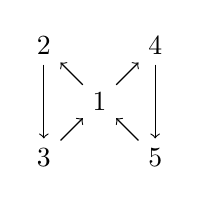
\begin{tikzpicture}
     \node (1) {1};
     \node[above left of=1](2){2};
     \node[below left of=1](3){3};
     \node[above right of=1](4) {4};
     \node[below right of=1](5) {5};
     \draw[->]
     (1) edge (2)
     (2) edge (3)
     (3) edge (1)
     (1) edge (4)
     (4) edge (5)
     (5) edge (1);
     \end{tikzpicture}
     \]

\begin{enumerate}
\item Find \(A^{24}_{1,1}\).
\begin{workbox}
\(A^{24}_{1,1} =\) 
\end{workbox}

\item Write one \((i,j)\) for which \(A^{26}_{i,j}\) is zero and one for which it is non-zero.
\begin{workbox}
\(A^{26}_{i,j} = 0\) for \((i,j) =\)
\hfill
\(A^{26}_{i,j} \neq 0\) for \((i,j) =\)
\hfill
\hspace{3cm}
\end{workbox}
\end{enumerate}

\item (2 points) Draw a connected directed graph on at least 3 vertices for which \(A^3 = 0\) but \(A^2 \neq 0\).

\begin{workbox}
\vspace{3cm}
\end{workbox}
\end{enumerate}

\newpage
\begin{enumerate}
\item Solutions
\label{sec:org3dc2888}
\begin{enumerate}
\item \begin{enumerate}
\item False.  It is the number of paths of length exactly \(k\).
\item True.  A long enough path must include a cycle.
\item True.  The only way \(A^4 \neq 0\) is if there is a cycle.  And in that case, \(A^5 \neq 0\) as well.
\item True.  Paths of length \(2\) and \(3\) from \(1\) to \(1\) give paths of length \(2+2, 2+3, 3+3, 2+2+3,\) etc.
\end{enumerate}
\item \begin{enumerate}
\item The only way to go from \(1\) to \(1\) is by following the left half of the bowtie or the right half of the bowie, both of which are of length 3.  In path of length 24, there will be 8 iterations of left/right bowtie, and each can be chosen independently leading to \(2^8 = 256\) possibilities.

\item \(A^{26}_{i,j} = 0\) for \((i,j) = (1,1)\), for example and \(A^{26}_{i,j} \neq 0\) for \((i,j) = (1,3)\). Lengths of paths from \(1\) to \(1\) are always divisible by 3; lengths of paths from \(1\) to \(2\) are \(1 \pmod 3\); from \(1\) to \(3\) are \(2 \pmod 3\), etc.
\end{enumerate}

\item Many possibilities, for example: \(1 \to 2 \to 3\).
\end{enumerate}
\end{enumerate}
\subsection{Quiz in week 6}
\label{sec:org6d477bb}
The quiz is in-class; nothing to see here.  This is just to record the scores.
\href{https://canvas.anu.edu.au/files/847946/download?download\_frd=1\&verifier=wfv6aQrbvmhQAz4zlucmJqQqWL3xN7YycBYkmxVv}{See the quiz (with solutions) here.}
\subsubsection{Quiz 5}
\label{sec:org7a3b74c}
\thispagestyle{empty}

\begin{center}
\begin{tabular}{ll}
\textbf{Name:} & \makebox[0.7\linewidth]{\hrulefill}\\
 & \\
\textbf{UID:} & \makebox[0.7\linewidth]{\hrulefill}\\
\end{tabular}
\end{center}
\vspace{1em}

Justifications are not required in any of the questions.

\begin{enumerate}
\item (5 points) True or false?

\begin{enumerate}
\item Let \(G\) be a weighted directed graph with \(5\) vertices.
(Each weight is a non-negative number and all loops are included with weight 0.)
If \(W\) is its weighted adjacency matrix, then the minimum cost to travel from vertex \(2\) to vertex \(3\) is the \((2,3)\) entry of \(W^{\odot 7}\).

\hfill \(\fbox{\phantom X}\) True \hfill \(\fbox{\phantom X}\) False \hfill.

\item Let \(A\) be the boolean adjacency matrix of a directed graph.
If \(n\) is large enough, then \(A^{*n} = A^{*(n+1)} = A^{*(n+2)} = \cdots\).

\hfill \(\fbox{\phantom X}\) True \hfill \(\fbox{\phantom X}\) False \hfill.

\item Let \(W\) be a matrix.  Let \(\oplus\) denote the min-plus addition.
Then \(W \oplus W = W\).

\hfill \(\fbox{\phantom X}\) True \hfill \(\fbox{\phantom X}\) False \hfill.

\item Let \(A\) be a boolean matrix.  There always exists a boolean matrix \(B\) such that \(A+B\) is the zero matrix.

\hfill \(\fbox{\phantom X}\) True \hfill \(\fbox{\phantom X}\) False \hfill.

\item Let \(A\) be a boolean matrix and let \(I\) be the identity matrix considered as a boolean matrix.
Then \((I+A)^{*2} = I + A + A^{*2}\).

\hfill \(\fbox{\phantom X}\) True \hfill \(\fbox{\phantom X}\) False \hfill.
\end{enumerate}

\item (3 points)  Let \(W\) be the weighted adjacency matrix of the following graph.
\begin{center}
\includegraphics[width=0.3\textwidth]{2c.png}
\label{orgf906720}
\end{center}
Find \(W^{\odot 10}\).
\begin{workbox}
\vspace{2cm}
\end{workbox}

\item (2 points) Find \(W \oplus W^{\odot 2} \oplus \cdots \oplus W^{\odot 2025}\). 
\begin{workbox}
\vspace{2cm}
\end{workbox}
\end{enumerate}
\begin{enumerate}
\item Solutions
\label{sec:orgee5b5b1}
\begin{enumerate}
\item \begin{enumerate}
\item True.
\item False (for example, take a 3-cycle \(1 \to 2 \to 3 \to 1\)).
\item True.
\item False (in fact, this almost never happens).
\item True.
\end{enumerate}

\item \[ W^{\odot 10} = \begin{pmatrix} 1 &1.9 \\ 2.9 & 1 \end{pmatrix}\]

\item \[ W + \dots + W^{\odot 2025} = \begin{pmatrix} 0.1 & 1 \\ 2 & 0.1  \end{pmatrix}\]
\end{enumerate}
\end{enumerate}
\subsection{Quiz in week 7}
\label{sec:org8e5035f}
The quiz is in-class; nothing to see here.  This is just to record the scores.

\href{https://canvas.anu.edu.au/files/866126/download?download\_frd=1\&verifier=svQh2A2xUQdOmC9ns5pl5yDZObJIB6VPDdAK4J5G}{Here is the quiz (with solutions).}
\subsubsection{Quiz 6}
\label{sec:org3312c61}
\thispagestyle{empty}

\begin{center}
\begin{tabular}{ll}
\textbf{Name:} & \makebox[0.7\linewidth]{\hrulefill}\\
 & \\
\textbf{UID:} & \makebox[0.7\linewidth]{\hrulefill}\\
\end{tabular}
\end{center}
\vspace{1em}

Justifications are not required in any of the questions.

\begin{enumerate}
\item (4 points) State true or false.
\begin{enumerate}
\item Let \(A\) be the transition matrix of a the following Markov chain: \phantom{here}
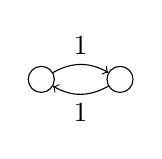
\begin{tikzpicture}[baseline=0cm]
\draw[->] node[draw,circle] (1) {} node[draw,circle, right of=1] (2) {}
(1) edge[bend left=30] node[above] {1} (2)
(2) edge[bend left=30] node[below] {1} (1);
\end{tikzpicture}

Then \(A^{5}\) is the identity matrix.

\medskip

\hfill \(\fbox{\phantom X}\) True \hfill \(\fbox{\phantom X}\) False \hfill.

\item Let \(A\) be the transition matrix of a Markov chain with a strongly connected graph.
Then \(\lim_{n\to\infty} A^{n}\) must exist.

\medskip

\hfill \(\fbox{\phantom X}\) True \hfill \(\fbox{\phantom X}\) False \hfill.

\item The Markov chain below satisfies the Perron-Frobenius property
\[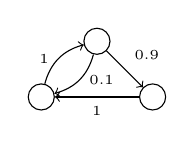
\begin{tikzpicture}
      \draw[->] node[draw,circle] (1) {}
      node[draw,circle,below left of=1] (2) {}
      node[draw,circle,below right of=1] (3) {}
      (1) edge[bend left=30] node[right] {\tiny 0.1} (2)
      (2) edge[bend left=30] node[left] {\tiny 1} (1)
      (1) edge node[above right] {\tiny 0.9} (3)
      (3) edge node[below] {\tiny 1} (2);
      \end{tikzpicture}
      \]
\hfill \(\fbox{\phantom X}\) True \hfill \(\fbox{\phantom X}\) False \hfill.

\item Let \(A\) be the transition matrix of a Markov chain.
If \(\lim_{n \to \infty} A^n\) exists, then all its rows are equal.

\medskip

\hfill \(\fbox{\phantom X}\) True \hfill \(\fbox{\phantom X}\) False \hfill.
\end{enumerate}

\item (3 points) Let \(A\) be the transition matrix of the Markov chain.
\[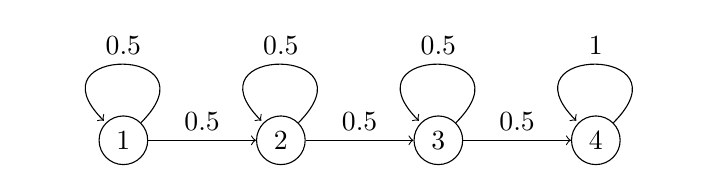
\begin{tikzpicture}[node distance=2cm]
   \draw node[draw,circle] (1) {1} node[draw,circle, right of=1] (2) {2} node [draw,circle,right of=2] (3) {3} node [draw,circle,right of=3] (4) {4};
     \draw[->] (1) edge node[above] {\(0.5\)} (2)
     (2) edge node[above] {\(0.5\)} (3)
     (3) edge node[above] {\(0.5\)} (4)
     (1) edge [loop] node[above] {\(0.5\)} (1)
     (2) edge [loop] node[above] {\(0.5\)} (2)
     (3) edge [loop] node[above] {\(0.5\)} (3)
     (4) edge [loop] node[above] {\(1\)} (4);    
   \end{tikzpicture} \]
\begin{workbox}
\vspace{0.5cm}

A\textsuperscript{2}\textsubscript{1,1} = \hfill A\textsuperscript{2}\textsubscript{1,4} = \hfill A\textsuperscript{3}\textsubscript{1,4} = \hfill.

\vspace{0.5cm}
\end{workbox}

\item (3 points) In the same Markov chain above, let \(B = \lim_{n \to \infty} A^n\) (this exists).  
\begin{workbox}
\vspace{0.5cm}

B\textsubscript{4,4} = \hfill B\textsubscript{1,1} = \hfill B\textsubscript{3,4} =  \hfill.

\vspace{0.5cm}
\end{workbox}
\end{enumerate}
\begin{enumerate}
\item Solutions
\label{sec:org9fe7144}
\begin{enumerate}
\item True or false
\begin{enumerate}
\item False (it has 1s on the anti-diagonal and 0s on the diagonal)
\item False (the above example is a counter-example)
\item True
\item False.  For example, consider our win-by-2 game.
\end{enumerate}
\item \begin{itemize}
\item \(A^2_{1,1} = 0.5^2 = 0.25\)
\item \(A^2_{1,4} = 0\)
\item \(A^3_{1,4} = (0.5)^3 = 0.125.\)
\end{itemize}
\item \begin{itemize}
\item \(B_{4,4} = 1\)
\item \(B_{1,1} = 0\)
\item \(B_{3,4} = 1\).

This is probably the least obvious.  But it is obvious that \(B_{3,1} = B_{2,1} = 0\).  And by the same logic as \(B_{4,4} = 0\), we get \(B_{3,3} = 0\).  Since the rows have to sum up to 1, we must have \(B_{3,4} = 1\).

A more direct way to see it is to observe that
\[ A^n_{3,4} = 0.5 + 0.5^2 + \cdots + 0.5^{n-1}.\]
So \(B_{3,4} = 0.5 + 0.5^2 + \cdots  = 1.\)
\end{itemize}
\end{enumerate}
\end{enumerate}
\subsection{Quiz in week 8}
\label{sec:orgab70f27}
The quiz is in-class; nothing to see here.  This is just to record the scores.

\href{https://canvas.anu.edu.au/files/866148/download?download\_frd=1\&verifier=yEVyjyFHeBSCDBgUOidjIOuafYIYOQTqZeT5K6LT}{Here is the quiz with solutions.}
\subsubsection{Quiz 7}
\label{sec:orgbb5eb27}
\thispagestyle{empty}

\begin{center}
\begin{tabular}{ll}
\textbf{Name:} & \makebox[0.7\linewidth]{\hrulefill}\\
 & \\
\textbf{UID:} & \makebox[0.7\linewidth]{\hrulefill}\\
\end{tabular}
\end{center}
\vspace{1em}

\begin{enumerate}
\item (6 points) Select either true or false. Let \(\Sigma = \{0,1\}\).
\begin{enumerate}
\item The string \(010001\) matches the regular expression \((0(0|1))^{\ast}\).

\hfill \(\fbox{\phantom X}\) True \hfill \(\fbox{\phantom X}\) False \hfill.

\item The string \(110\) matches the regular expression \((\epsilon | 0)1^{*}0\)

\hfill \(\fbox{\phantom X}\) True \hfill \(\fbox{\phantom X}\) False \hfill.

\item If \(r_1 = 01^{\ast}\) and \(r_2 = (01)^{\ast}\), then \(L(r_1) = L(r_2)\).

\hfill \(\fbox{\phantom X}\) True \hfill \(\fbox{\phantom X}\) False \hfill.

\item If \(r_1 = 0(1^{\ast}|0^{\ast})0\) and \(r_2 = (01^{\ast}0)|(000^{\ast})\) then \(L(r_1) = L(r_2)\).

\hfill \(\fbox{\phantom X}\) True \hfill \(\fbox{\phantom X}\) False \hfill.

\item Any DFA must have at least one accept state.

\hfill \(\fbox{\phantom X}\) True \hfill \(\fbox{\phantom X}\) False \hfill.

\item Any DFA must have at most one accept state.   

\hfill \(\fbox{\phantom X}\) True \hfill \(\fbox{\phantom X}\) False \hfill.
\end{enumerate}

\item (2 points)
Write down a regular expression whose language is exactly all those words in \(\Sigma^{\ast}\) that contain the string \(101\) as a (contiguous) substring.
\begin{workbox}
\vspace{2cm}
\end{workbox}

\item (2 points)
Draw a DFA whose language is \(10^{\ast}\).
\begin{workbox}
\vspace{4cm}
\end{workbox}
\end{enumerate}
\begin{enumerate}
\item Solutions
\label{sec:orgbf7afbd}
\begin{enumerate}
\item \begin{enumerate}
\item True
\item True
\item False
\item True
\item False
\item False
\end{enumerate}

\item \((0|1)^{*}101(0|1)^{*}\)

\item Here is a DFA.

\begin{center}
\includegraphics[width=.3\textwidth]{assets/Quizzes/2025-09-29_11-46-56_screenshot.png}
\end{center}
\end{enumerate}
\end{enumerate}
\subsection{Quiz in week 9}
\label{sec:org305d3af}
The quiz is in-class; nothing to see here.  This is just to record the scores.

\href{https://canvas.anu.edu.au/files/1193063/download?download\_frd=1\&verifier=2jjBzNfXRx1mDfFXAq0PmNgeE1S7kWX5d5pb2ZqB}{Here is the quiz with solutions.}
\subsubsection{Quiz 8}
\label{sec:org38c8232}
\thispagestyle{empty}

\begin{center}
\begin{tabular}{ll}
\textbf{Name:} & \makebox[0.7\linewidth]{\hrulefill}\\
 & \\
\textbf{UID:} & \makebox[0.7\linewidth]{\hrulefill}\\
\end{tabular}
\end{center}
\vspace{1em}

\begin{enumerate}
\item (4 points) Select either true or false. 
\begin{enumerate}
\item In an NFA, arrows are allowed to have \(\epsilon\) as a label.

\hfill \(\fbox{\phantom X}\) True \hfill \(\fbox{\phantom X}\) False \hfill.

\item Every NFA is also a DFA.

\hfill \(\fbox{\phantom X}\) True \hfill \(\fbox{\phantom X}\) False \hfill.

\item For an NFA with \(5\) states, there exists an equivalent DFA that has at most \(32\) states.

\hfill \(\fbox{\phantom X}\) True \hfill \(\fbox{\phantom X}\) False \hfill.

\item There is a regular expression whose language is not recognised by any DFA.

\hfill \(\fbox{\phantom X}\) True \hfill \(\fbox{\phantom X}\) False \hfill.
\end{enumerate}

\item (6 points) Consider the NFA shown below.
\begin{center}
  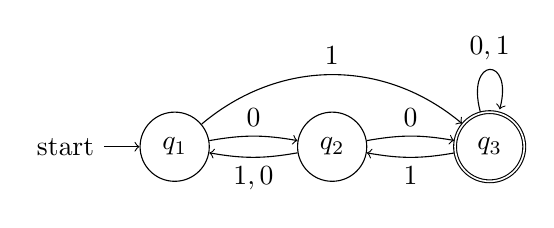
\begin{tikzpicture}[node distance=2cm]
    \node[state,initial] (q1) {$q_1$};
    \node[state] (q2) [right of=q1] {$q_2$};
    \node[state, accepting] [right of=q2](q3) {$q_3$};
    \path[->]
    (q1) edge[bend left=10] node[above] {$0$} (q2)
    (q1) edge[bend left=40] node[above] {$1$} (q3)
    (q2) edge[bend left=10] node[below] {$1,0$} (q1)
    (q2) edge[bend left=10] node[above]{$0$} (q3)
    (q3) edge[bend left=10] node[below]{$1$} (q2)
    (q3) edge[loop above] node {$0,1$} ()
    ;
  \end{tikzpicture}
\end{center}
Describe the complete run of the NFA on the input string \(w = 0010\).
The \(n\)th step in your description should be the set of all possible states after reading \(n\) letters of \(w\).
Write whether the string is accepted or rejected.
\begin{workbox}
\vspace{7.5cm}
\end{workbox}
\end{enumerate}
\begin{enumerate}
\item Solutions
\label{sec:org055cfba}
\begin{enumerate}
\item True or false
\begin{enumerate}
\item True
\item False
\item True
\item False
\end{enumerate}

\item \mbox{}\\

\begin{center}
\begin{tabular}{rl}
Step & Possibile states\\
\hline
0 & \(q_1\)\\
1 & \(q_2\)\\
2 & \(q_1,q_3\)\\
3 & \(q_2,q_3\)\\
4 & \(q_1, q_3\)\\
\end{tabular}
\end{center}

Since \(q_3\) is an accept state, the string is accepted.
\end{enumerate}
\end{enumerate}
\subsection{Quiz in week 10}
\label{sec:org08e902e}
The quiz is in-class; nothing to see here.  This is just to record the scores.
\subsubsection{Quiz 9}
\label{sec:orge594bc8}
\thispagestyle{empty}

\begin{center}
\begin{tabular}{ll}
\textbf{Name:} & \makebox[0.7\linewidth]{\hrulefill}\\
 & \\
\textbf{UID:} & \makebox[0.7\linewidth]{\hrulefill}\\
\end{tabular}
\end{center}
\vspace{1em}
\begin{enumerate}
\item (6 points) Select either true or false.

\begin{enumerate}
\item The intersection of two regular languages is a regular language.\\

\hfill \(\fbox{\phantom X}\) True \hfill \(\fbox{\phantom X}\) False \hfill.

\item If the intersection of two languages is regular, then both of those languages have to be regular.\\

\hfill \(\fbox{\phantom X}\) True \hfill \(\fbox{\phantom X}\) False \hfill.

\item If the smallest DFA that recognises \(L\) has \(100\) states, then the pumping lemma says nothing about strings of length \(90\).\\

\hfill \(\fbox{\phantom X}\) True \hfill \(\fbox{\phantom X}\) False \hfill.

\item If a language is recognised by a DFA with 4 states, then the Myhill-Nerode equivalence relation has 4 equivalence classes.\\

\hfill \(\fbox{\phantom X}\) True \hfill \(\fbox{\phantom X}\) False \hfill.

\item Let \(L = \{0^n1^{n} \mid n = 1,2,3,\cdots,\}\).
A pumping lemma argument implies that any 10-state DFA that accepts \(0^{11}1^{11}\) must also accept \(0^{12}1^{12}\).\\

\hfill \(\fbox{\phantom X}\) True \hfill \(\fbox{\phantom X}\) False \hfill.

\item Let \(L\) be a language and \(L^c\) its complement.
If \(x \sim_L y\) then \(x \sim_{L^c} y\).\\

\hfill \(\fbox{\phantom X}\) True \hfill \(\fbox{\phantom X}\) False \hfill.
\end{enumerate}

\item (4 points) Let \(L\) be the language on the alphabet \(\{0,1\}\) consisting of strings that are at least 2 letters long and whose 2nd letter is \(1\).

\begin{enumerate}
\item Is \(L\) regular?

\hfill \(\fbox{\phantom X}\) Yes \hfill \(\fbox{\phantom X}\) No \hfill.

\item Write 4 strings that represent 4 distinct Myhill-Nerode equivalence classes for \(L\).
\begin{workbox}
\vspace{3cm}
\end{workbox}
\end{enumerate}
\end{enumerate}

\newpage
\begin{enumerate}
\item Solutions
\label{sec:org2be8f5d}
\begin{enumerate}
\item True or false.
\begin{enumerate}
\item True
\item False (for example, take the empty language and a non-regular language).
\item True.
\item False (at most 4)
\item False.
\item True.
\end{enumerate}

\item \mbox{}\\
\begin{enumerate}
\item Yes, it is regular (regex: \((0|1)1(0|1)^{*}\).
\item \(\epsilon, 0, 00, 01\).

\begin{itemize}
\item \(z = \epsilon\) distinguishes the fourth from the first three.
\item \(z = 1\) distinguishes \(0\) from \(\epsilon\) and \(00\).
\item \(z = 01\) distinguishes \(\epsilon\) from the later three.
\end{itemize}
\end{enumerate}
\end{enumerate}
\end{enumerate}
\subsection{Quiz in week 11}
\label{sec:orge778a34}
The quiz is in-class; nothing to see here.  This is just to record the scores.
\subsubsection{Quiz 10}
\label{sec:orgcb81de0}
\thispagestyle{empty}

\begin{center}
\begin{tabular}{ll}
\textbf{Name:} & \makebox[0.7\linewidth]{\hrulefill}\\
 & \\
\textbf{UID:} & \makebox[0.7\linewidth]{\hrulefill}\\
\end{tabular}
\end{center}
\vspace{1em}

\begin{enumerate}
\item (5 points) Select true or false
\begin{enumerate}
\item A game graph cannot have an edge from an \(N\) state to an \(N\) state.

\hfill \(\fbox{\phantom X}\) True \hfill \(\fbox{\phantom X}\) False \hfill.

\item A game graph cannot have an edge from a \(P\) state to a \(P\) state.

\hfill \(\fbox{\phantom X}\) True \hfill \(\fbox{\phantom X}\) False \hfill.

\item If a state is labelled \(N\), then the next player will win, no matter which move they make.

\hfill \(\fbox{\phantom X}\) True \hfill \(\fbox{\phantom X}\) False \hfill.

\item \(10 \times 10\) Chomp is an \(N\) game.

\hfill \(\fbox{\phantom X}\) True \hfill \(\fbox{\phantom X}\) False \hfill.

\item If \(G\) is an \(N\) game, then \(G+G\) is a \(P\) game.

\hfill \(\fbox{\phantom X}\) True \hfill \(\fbox{\phantom X}\) False \hfill.
\end{enumerate}

\item (5 points) 
Remember the rules of Grundy's game: we start with piles of stones and a move consists of dividing a pile in two non-empty piles of unequal sizes.  Draw the game graph of Grundy's game starting with two piles of size \(3\) and \(4\).  Label each node as \(N\) or \(P\).
\end{enumerate}

\newpage
\begin{enumerate}
\item Solutions
\label{sec:org1173a23}
\begin{enumerate}
\item True or false
\begin{enumerate}
\item False.
\item True.
\item False.
\item True.
\item True.
\end{enumerate}

\item The game graph has the following edges
\begin{align*}
  (3,4) &\to (1,2,4) \text{ and } (3,1,3)\\
  (1,2,4) &\to (1,2,1,3)\\
  (3,1,3) &\to (1,2,1,3)\\
  (1,2,1,3) &\to (1,2,1,1,2).
\end{align*}
This means \((1,2,1,1,2)\) is \(P\); \((1,2,1,3)\) is \(N\); both \((1,2,4)\) and \((3,1,3)\) are \(P\); and \((3,4)\) is \(N\).
\end{enumerate}
\end{enumerate}
\subsection{Quiz in week 12}
\label{sec:org7356a37}
The quiz is in-class; nothing to see here.  This is just to record the scores.
\section{EAP}
\label{sec:orgea336a4}

\subsection{Luca Moses}
\label{sec:org1493f25}
Flexible attendance (should not be penalised for missing workshops).
\href{mu4e:msgid:ME3P282MB219424DF74C3D4E63B1D5AD7A32EA@ME3P282MB2194.AUSP282.PROD.OUTLOOK.COM}{EAP and MATH2301}
\subsection{Maxibonn}
\label{sec:org65c7162}
\begin{itemize}
\item Different seating arrangements (quieter/more secluded)
\end{itemize}
\section{Final exam preparation}
\label{sec:org5f03410}
\subsection{Practice problems}
\label{sec:org957051b}
\subsubsection{Shorter questions to test basic understanding}
\label{sec:org4b44545}
These are quick/slightly open-ended questions that you should be able to answer if you have been keeping up to date with lectures. These are good to do in discussion with classmates.

Don't be tempted to skip these! If you can easily answer all these questions, you should consider yourself fairly well-prepared in the theory required for the examination. Conversely, if you struggle with these, it is important that you come to office hour or drop-in sessions to see where you need to catch up.

\begin{enumerate}
\item How many subsets does the empty set have?
\item How many elements are in \(\emptyset \times \{3,4,5\}\)?
\item How many possible relations are there on the set \(\{1,2,3\}\)?
\item Consider the relation \(\{(a,b) \mid a \mid b\}\) on \(\mathbb{N}\). Is this the I/O relation of a function on \(\mathbb{N}\)?
\item Do you know how to draw the graph of a relation on a set?
\item If \(A\) is a \(4 \times 5\) matrix and \(B\) is a \(2 \times 4\) matrix, does the matrix product \(AB\) make sense?
\item What do you know about the adjacency matrix of a relation if the relation is reflexive/symmetric?
\item How many different equivalence classes in modular arithmetic do you have if the modulus is \(2020\)?
\item Let \(G\) be a directed graph with \(10\) vertices. Let \(a\) and \(b\) be vertices that are connected by at least one path from \(a\) to \(b\). Can the shortest path from \(a\) to \(b\) have length \(12\)?
\item Is it always the case that the boolean powers of an adjacency matrix stabilise after a certain point? If yes, justify. If not, find a counterexample.
\item Is it always the case that the min-plus powers of a weighted adjacency matrix stabilise after a certain point? If yes, justify. If not, find a counterexample.
\item Do you understand how to check whether an expression is a valid regex? What are the atomic regexes and what are the basic operations?
\item Is \(1^{k}\) a valid regex in the alphabet \(\Sigma = \{0,1\}\)? Why or why not?
\item What is the difference between \((01)^{\ast}\) and \((0|1)^{\ast}\)? What about \(01^{\ast}\)?
\item Write down the concatenated language of \(L_1 = \{11,01\}\) and \(L_2 = \{00\}\).
\item Write down the concatenated language of \(L_3 = \{0,1,11,01\}\) and \(L_4 = \emptyset\).
\item For each of the pairs above, write down the union language.
\item What is the difference between DFAs and NFAs?
\item What does it mean for an NFA to accept or reject a string?
\item Did you understand the construction of a product automaton? Why did we fail at directly constructing DFAs for the concatenation, or, and star operations?
\item Given a regex \(r\), is it always possible to construct a DFA \(M\) such that \(L(M) = L(r)\)? (The answer is yes, but make sure you understand why.) In particular, if the answer is yes, why does it not contradict the fact that we failed at directly constructing DFAs for the concatenation, or, and star operation in class?
\item Are all languages regular?
\item Are all finite languages regular?
\item What is the Myhill--Nerode equivalence relation?
\item What does the number of equivalence classes of the Myhill--Nerode relatio have to do with the regularity of the language?
\item What is the winning strategy for a game of nim? Given a nim position, say \((3,4)\), can you figure out how many optimal moves there are?
\item Draw the game graph starting at the nim position of \((1,1,2)\). Label the graph \(N\) and \(P\) using the N/P labelling.
\item Draw the game graph of a \(3 \times 3\) game of chomp, and write down the Grundy label of each position.
\item Is the nim position \((12,13,14,15,16)\) an N position or a P position? What is the nim value of this position?
\item Do you remember what it means to add two games?
\item Do you remember what it means for two games to be equivalent? Why is this an equivalence relation?
\item Can you give an example of two games \(G_1\) and \(G_2\) that are both \(N\) positions but are not equivalent?
\item Can you give an example of two games \(G_1\) and \(G_2\) that are both \(P\) positions but are not equivalent?
\item If \(G_1\) and \(G_2\) are equivalent, must they have the same outcome?
\end{enumerate}
\subsubsection{Longer questions}
\label{sec:orgb75769c}
These questions are slightly longer. So you should try to solve these independently first, without consulting anyone else. Once you have attempted them, you can discuss with me or with classmates to check your work.
\begin{enumerate}
\item Consider the relation \(\{((a,b),(c,d)) \in \mathbb{R}^2 \times \mathbb{R}^2 \mid \operatorname{max}\{a,b\} = \operatorname{max}\{c,d\}\}\). Is this an equivalence relation? If yes, can you describe and draw the equivalence classes? If not, which of the three required properties does and doesn't it satisfy?
\item Show that if \(\sim\) is an equivalence relation on a set \(S\), then the equivalence classes of \(\sim\) partition the set \(S\). That is, the equivalence classes are disjoint subsets of \(S\) whose union is \(S\).
\item Show that the relation \(\{((a,b),(c,d)) \in \mathbb{R}^2 \times \mathbb{R}^2\mid b - a^2 = d - c^2\}\) is an equivalence relation. What are the equivalence classes? Can you draw them on the plane?
\item Consider equivalence under the modular relation (\(x \sim y\) if \(d \mid (x-y)\)) for \(d = 10\). How many different equivalence classes \([x]\) are there such that \([x^2] = [1]\)? How many are there such that \([x^3] = [1]\)?
\item Consider equivalence under the modular relation (\(x \sim y\) if \(d \mid (x-y)\)) for \(d = 12\).
Is it possible to find an equivalence class \([x]\) such that \([3]\cdot [x] = [1]\)? Why or why not?
\item Find an example of a graph such that when you order the vertices in two different ways, the adjacency matrix changes.
\item Find the transitive closure of the relation \(\{(a,b) \mid b = a\cdot p\text{ for some prime number }p\}\) on the set \(\{1,2,3,4,5,6\}\). See if you can check your answer using Boolean powers of the adjacency matrix. (Yes, I know it's a large matrix!)
\item Draw your favourite weighted directed graph on \(4\) vertices, and compute the least-cost path weights between any pair of vertices using min-plus powers of the weighted adjacency matrix.
\item Directly write down an NFA that recognises the concatenation of \(L_1 = 0^{*}\) and \(L_2 = 1^{*}\). Convert this to a DFA.  Can there be a smaller DFA (fewer states) than this?  How do you know?
\item Write down a product automaton for the union of the languages \(L_1\) and \(L_2\) above.
Then write down an equivalent automaton directly, without using a product construction.
Convert this to a DFA.  Can there be a smaller DFA (fewer states) than this?  How do you know?
\item Construct a DFA to recognise the following language:
\[L = \{w \mid \text{ the length of }w\text{ is at most }4\}.\]
\item Let \(F\) be the language of all strings over \(\{0,1\}\) that do not contain a pair of \(1\)s that are separated by an odd number of symbols. Give the state diagram of a DFA with five states that recognises \(F\).
You may find it helpful to first draw a four-state NFA that recognises the complement of \(F\).
\item Convert the regular expression \(01^*(01)^*|10\) into an equivalent NFA.
\item Convert the following DFA into an equivalent regular expression:
\begin{center}
  \begin{tikzpicture}[node distance=2cm]
    \node[state, initial, accepting] (q1) {$q_1$};
    \node[state] (q2) [right of=q1] {$q_2$};
    \node[state, accetping] (q3) [below of=q2] {$q_3$};
    \path[->]
    (q1) edge[loop above] node {$0$} ()
    (q1) edge node[above] {$1$} (q2)
    (q2) edge[loop above] node {$0$} ()
    (q2) edge node[right] {$1$} (q3)
    (q3) edge[loop right] node {$0,1$} ()
    ;
  \end{tikzpicture}
\end{center}
\item Recall what it means for two games to be equivalent; give some distinct nim positions that are equivalent to the nim game \((12,13,14,15,16)\) above.
\item Recall Wythoff's game: the game positions are given by a single queen on a chessboard. Players take turns moving the queen. The queen can only be moved vertically down, horizontally to the left, or diagonally down to the left.
When the queen reaches the lower left corner, the game is over and the player to move last wins.
Consider an \(8 \times 8\) chessboard and fill in the Grundy value of each square.
\item The game of take-a-prime is played as follows. The starting position is some positive integer \(n\). A move consists of removing a prime number from \(n\) (that is, any of the numbers \(\{2,3,5,7,11,\ldots\}\)). The player who cannot make a move loses. Draw the game graph and Grundy labels for the starting position of \(n = 15\).
\item Consider the game \(G + H\), where \(G\) is Grundy's game from the previous problem, with the starting position of \(n = 15\), and \(H\) is a nim game with starting position \((3,4,5)\).
What is the Grundy value of \(G + H\)? If it is positive, find an optimal move.
\item Consider nim with a starting position of \((7, 8, 9, 10)\). Figure out how many ways there are (if any) to go from this game position to a position with nim sum \(8\). Justify.
\item Consider the SOS game. The game board is a row of \(n\) squares, initially empty. Players take turns selecting an empty square and writing either an \(S\) or an \(O\) in it. The player who first succeeds in writing \(SOS\) in consecutive squares wins the game. If the board fills up with no \(SOS\) in it, the game is a draw. Show that if \(n = 4\) and the first player puts an \(S\) in the first square, then the second player can win.
\item Show that game addition satisfies the following property: if \(G\) and \(H\) are games, then \(G + G + H \sim H\).
\end{enumerate}
\subsection{Old midterm examination}
\label{sec:orgab6ac62}
\subsubsection{Questions}
\label{sec:org1eb1292}
\setenumerate{itemsep=1em}
\begin{enumerate}
\item Question 1
\label{sec:org376b5c8}
Answer the following true or false questions by clearly writing either ``True'' or ``False'' (not just T and F). Justifications are not required. The parts are worth 2 points each.
\begin{enumerate}
\item True or false: it makes sense to take the square of a \(3 \times 2\) matrix.
\item True or false: if \(G\) is a graph with \(10\) vertices and \(i,j\) are any two vertices of \(G\), then there must be a path of length at most \(10\) from \(i\) to \(j\).
\item True or false: if \(R\) is a partial order relation on a set \(S\) and \(a,b \in S\), then it is possible that \((a,b) \notin R\) and \((b,a) \notin R\).
\item True or false: in an equivalence relation, if \(b \in [a]\), then \([b] = [a]\).
\item True or false: any finite poset has a maximal element.
\end{enumerate}
\item Question 2
\label{sec:org0b64259}
Answer the following short questions. Justifications are not required. The parts are worth 3 points each.
\begin{enumerate}
\item Let \(A = \{1\}\) and \(B = \{a,b\}\).
Write down all elements of the power set of \(A \times B\).

\item Write down all possible relations on the set \(A = \{1\}\).

\item Consider the relation
\[\{(x,y) \in \mathbb{Z} \times \mathbb{Z} \mid (x - y)\text{ is a multiple of }12\}.\]
List all equivalence classes \([x]\) such that 
\[[x^2] = [1].\]

\item Recall that a \emph{minimum} element in a poset \(P\) is \(a \in P\) such that \(a \preceq b\) for every \(b \in P\).
Recall that a \emph{maximum} element in a poset \(P\) is \(a \in P\) such that \(a \succeq b\) for every \(b \in P\).

Draw the Hasse diagram for a poset that has both a minimum and a maximum element, but is not a total ordering.

\item Label the elements of the following poset in such a way that the matrix \(M_\zeta\) of the \(\zeta\) function is \uline{not} upper triangular.
Write down the matrix \(M_\zeta\) corresponding to your chosen labelling.
\begin{center}
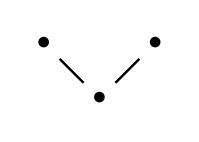
\begin{tikzpicture}
\node(A) at (0,0) {$\bullet$};
\node[above left of=A](B) {$\bullet$};
\node[above right of=A](C) {$\bullet$};
\draw[thick] (B) -- (A) -- (C);
\end{tikzpicture}         
\end{center}
\end{enumerate}
\item Question 3
\label{sec:orgece028a}
\begin{enumerate}
\item \emph{(3 points)} Write an example of a relation on \(\{1,2,3\}\) that is neither symmetric nor antisymmetric. Justification not required.
\item \emph{(3 points)} Write an example of a relation on \(\{1,2,3\}\) that is reflexive and symmetric, but not transitive. Justification not required.
\item \emph{(4 points)} Consider the equivalence relation
\[\{((a,b),(c,d)) \in \mathbb{R}^2 \times \mathbb{R}^2 \mid \min\{a,b\} = \min\{c,d\}\}.\]
Choose any \uline{specific} point \((a,b)\), and sketch its equivalence class.
Show your work.
\end{enumerate}
\item Question 4
\label{sec:org5097aa0}
For each relation, state whether or not the relation is an equivalence relation. Also state which of the required properties are and are not satisfied. Justify each property.
\begin{enumerate}
\item \emph{(5 points)} \(\{(a,b) \in \mathbb{Z} \times \mathbb{Z} \mid a + b \neq 1\}\)
\item \emph{(5 points)} Let \(S\) be any set and let \(T \subseteq S\) be a fixed subset. The relation \(\{(A,B) \in \mathcal{P}(S) \times \mathcal{P}(S) \mid A \cap T = B \cap T\}\).
\end{enumerate}
\item Question 5
\label{sec:orgd70139d}
Consider the equivalence relation
\[\{(x,y) \in \mathbb{Z} \times \mathbb{Z} \mid (x - y) \text{ is a multiple of }15\}.\]
\begin{enumerate}
\item \emph{(1 points)} How many distinct equivalence classes are there? Justification not required.

\item \emph{(3 points)} Find an integer \(x\) such that \(0 \leq x \leq 14\), with \([-31] = [x]\). Justify briefly.

\item \emph{(3 points)}
Consider the equation \([4] -  [x] = [21]\).
Is there an integer \(x\) that satisfies this equation?
If not, justify why.
If yes, find a positive integer that satisfies this, showing your work.

\item \emph{(3 points)}
Consider the equation \([2]\cdot [x] = [7]\). Find a positive integer that satisfies this, showing your work.
\end{enumerate}
\item Question 6
\label{sec:orgfdb5462}
\begin{enumerate}
\item \emph{(3 points)} Draw (as a graph) a relation on three vertices that is not reflexive, whose transitive closure is reflexive.
Also draw the graph of the transitive closure.
Justification not required.

\item \emph{(4 points)} Find the transitive closure of the following relation by using Boolean multiplication. It is sufficient to express your answer as an adjacency matrix.
\begin{center}
\includesvg[width=0.3\textwidth]{midterm-q3}
\label{orga86d1b4}
\end{center}
\end{enumerate}
\item Question 7
\label{sec:orgcdcd773}
Consider the weighted adjacency matrix
\[W =\begin{pmatrix}
  0  &  5  &  \infty  &  \infty \\
  \infty  &  0  &  1  &  \infty \\
  8  &  \infty  &  0  &  3 \\
  \infty  &  2  &  \infty  &  0 
\end{pmatrix}.\]
\begin{enumerate}
\item \emph{(3 points)} Draw the graph and edge weights corresponding to this weighted adjacency matrix, labelling your vertices \((1,2,3,4)\) in the order of the matrix rows/columns. Justification not required.

\item \emph{(5 points)} Using min-plus product, find the matrix showing the minimum cost of paths of any length between all pairs of vertices.
Show your work.
\end{enumerate}
\end{enumerate}
\subsection{Old final examination}
\label{sec:orgf237f97}
\toggletrue{solutions}
\subsubsection{Questions}
\label{sec:org8b48089}
\begin{enumerate}
\item Question (20 points total)
\label{sec:org0d5eb60}
Clearly write either ``True'' or ``False'' (not both!) for each of the statements below. No justification necessary.
\begin{enumerate}
\item The relation \(\{(a,b) \in \mathbb{N} \times \mathbb{N} \mid b - a = 1\}\) is a partial order relation.
\begin{solution}
False (not transitive)
\end{solution}

\item There is an integer \(a\) such that \(a^2 \equiv 3\) modulo \(11\).
\begin{solution}
True (for example, \(a = 5\)).
\end{solution}

\item The following Hasse diagram has a maximum element.
\begin{center}
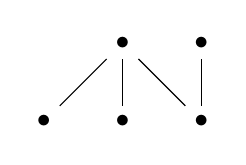
\begin{tikzpicture}
   \node (a) {$\bullet$};
   \node (b) [right of=a] {$\bullet$};
   \node (c) [right of=b] {$\bullet$};
   \node (d) [above of=b] {$\bullet$};
   \node (e) [above of=c] {$\bullet$};
   \draw (a) -- (d);
   \draw (b) -- (d);
   \draw (c) -- (d);
   \draw (c) -- (e);
\end{tikzpicture}
\end{center}
\begin{solution}
False.
\end{solution}

\item The language consisting of all strings such that no two \(1\)s in the string appear in consecutive positions is a regular language.
\begin{solution}
True (it is the complement of the language of \(r = \Sigma^{*}11\Sigma^{*}\)).
\end{solution}

\item Let \(L\) be a regular language. Then there is a unique DFA \(M\) such that \(L = L(M)\).
\begin{solution}
False.
\end{solution}

\item An NFA must have at least one accept state.
\begin{solution}
False.
\end{solution}

\item The game graph of the game state of an impartial combinatorial game has no directed loops.
\begin{solution}
True.
\end{solution}

\item If a game has Grundy label \(6\), then it is equivalent to a nim game whose state is \(4,3,1\).
\begin{solution}
True (the nim sum of the second nim game is \(100_2 + 11_2 + 1_2 = 110_2 = 6\)).
\end{solution}

\item In an impartial combinatorial game \(G\), it may be possible to move directly from a \(P\) position to another \(P\) position.
\begin{solution}
False (a \(P\) position is one that only maps to \(N\) positions).
\end{solution}
\end{enumerate}
\item Question (15 points total)
\label{sec:orge795eaf}
Answer the following short questions. No justifications are required.
\begin{enumerate}
\item Write down an example of an adjacency matrix \(A\) whose Boolean powers do not stabilise.
In other words, there is no \(n\) for which \(A^{\ast n} = A^{\ast m}\) for all \(m \geq n\).
\begin{solution}
One possible answer is
\[A = \begin{pmatrix}0 & 1\\1 & 0\end{pmatrix}.\]
\end{solution}

\item Let \(L_1 = \{010, 000\}\) and \(L_2 = \{1,\varepsilon\}\). List all elements of \(L_1 \circ L_2\).
\begin{solution}
The answer is \(\{0101, 0001, 010, 000\}\).
\end{solution}

\item How many winning moves are there in the nim game with position \((1, 2, 3,7)\)? List them all.
\begin{solution}
Eat the entire pile containing \(7\) berries.
\end{solution}
\end{enumerate}
\item Question (10 points total)
\label{sec:org1a5110a}
Consider the graph shown below.
\begin{center}
\includegraphics[width=0.6\textwidth]{final-12.png}
\label{org1ade35b}
\end{center}
\begin{enumerate}
\item (3 points) Draw the transitive closure of this graph, ignoring the weights. Justification not required.
\begin{solution}
\begin{center}
\includegraphics[width=.2\textwidth]{final-transitive.png}
\end{center}
\end{solution}

\item (7 points) Write down the weighted adjacency matrix using the weights shown in the diagram. Paths of length zero are considered to have weight zero. Calculate the matrix that shows the minimum weight paths between any pair of vertices. Show your work, clearly indicating any formulas that you used.
\begin{solution}
The weighted adjacency matrix is
\[ W = \begin{pmatrix}
   0&1&1&\infty\\
   \infty&0&3&\infty\\
   \infty&\infty&0&2\\
   1&5&\infty&0
   \end{pmatrix}. \]
The minimum-weight path can be computed by the min-plus cube of this matrix.
We have
\[W^{\odot 2} = 
   \begin{pmatrix}
   0&1&1&3\\
   \infty&0&3&5\\
   3&7&0&2\\
   1&2&2&0
   \end{pmatrix},
   \]

and
\[W^{\odot 3}
   \begin{pmatrix}
   0&1&1&3\\
   6&0&3&5\\
   3&4&0&2\\
   1&2&2&0        
   \end{pmatrix}.\]
\end{solution}
\end{enumerate}
\item Question (10 points total)
\label{sec:org13c05a1}
Consider the language \(L = \{0,1\}\) on the alphabet \(\Sigma = \{0,1\}\).
\begin{enumerate}
\item (3 points) Write down a \(3\)-state NFA that recognises \(L\). Justification is not required.
\begin{solution}
Here is a possible answer.
\begin{center}
  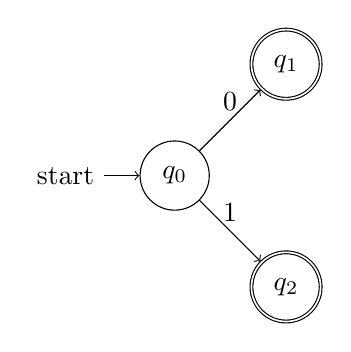
\begin{tikzpicture}[node distance=2cm]
    \node[state, initial](q0) {$q_0$};
    \node[state, accepting] (q1) [above right of=q0] {$q_1$};
    \node[state, accepting] (q2) [below right of=q0] {$q_2$};
    \path[->]
    (q0) edge node[above]{0} (q1)
    (q0) edge node[above]{1} (q2);
  \end{tikzpicture}
\end{center}
\end{solution}
\item (7 points) Convert your NFA to a DFA using the construction discussed in class.
It is sufficient to draw the final DFA as long as it is clearly labelled; no other justification is required.
\begin{solution}
We convert the previous NFA into a DFA. It will have \(8\) states.
      \begin{center}
        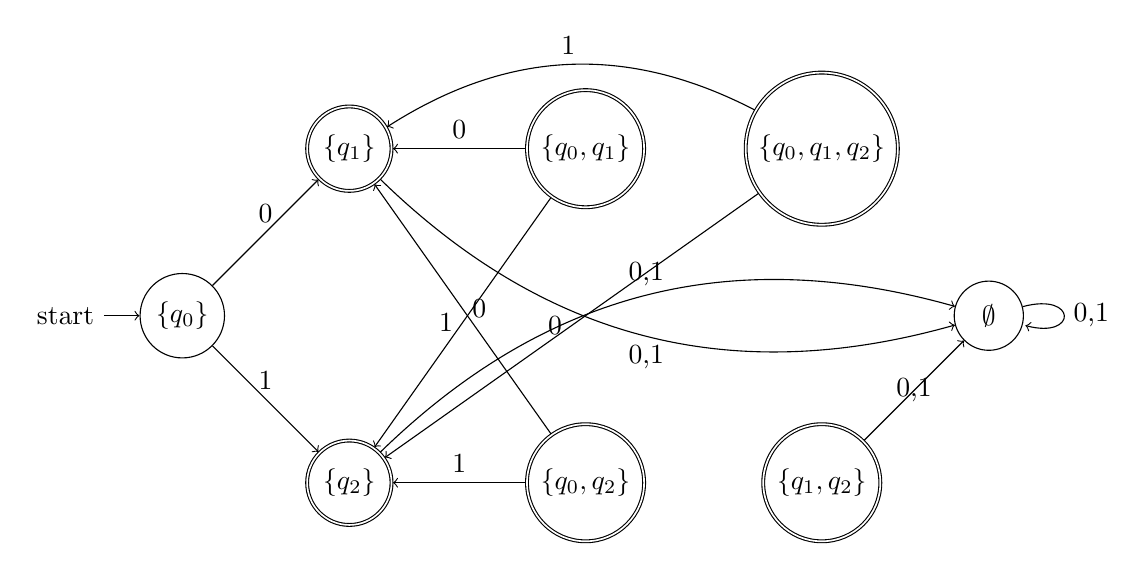
\begin{tikzpicture}[node distance=3cm]
          \node[state, initial](q0) {$\{q_0\}$};
          \node[state, accepting] (q1) [above right of=q0] {$\{q_1\}$};
          \node[state, accepting] (q0q1) [right of=q1] {$\{q_0, q_1\}$};
          \node[state, accepting] (q2) [below right of=q0] {$\{q_2\}$};
          \node[state, accepting] (q0q2) [right of=q2] {$\{q_0, q_2\}$};
          \node[state, accepting] (q0q1q2) [right of=q0q1] {$\{q_0, q_1, q_2\}$};
          \node[state, accepting] (q1q2) [right of=q0q2] {$\{q_1, q_2\}$};
          \node[state](e)[above right of=q1q2] {$\emptyset$};
          \path[->]
          (q0) edge node[above]{0} (q1)
          (q0) edge node[above]{1} (q2)
(q1) edge[bend right] node[below]{0,1} (e)
(q2) edge[bend left] node[above]{0,1} (e)
(q0q1) edge node[above]{0} (q1)
(q0q1) edge node[left]{1} (q2)
(q0q2) edge node[right]{0} (q1)
(q0q2) edge node[above]{1} (q2)
(q0q1q2) edge[bend right] node[above]{1} (q1)
(q0q1q2) edge node[left]{0} (q2)
(q1q2) edge node{0,1} (e)
(e) edge[loop right] node[right] {0,1} ();
        \end{tikzpicture}
      \end{center}
\end{solution}
\end{enumerate}
\item Question (10 points total)
\label{sec:orgb417a9e}
Let \(\Sigma = \{0,1\}\).
Suppose that \(r\) is some regular expression and \(L(r)\) is the language recognised by \(r\).
Let \(L'\) be the language
\[L' = \{(x_1 y_1 x_2 y_2 \ldots x_k y_k) \mid \text{ for some } k \geq 0, \text{ such that }x_i \in \Sigma^\ast\text{ and } y_j \in L(r)\text{ for each }i,j\}.\]
\begin{enumerate}
\item (3 points) Write down a regular expression that recognises \(L'\), in terms of \(r\).
That is, your answer is allowed to contain \(r\). Justify your answer briefly.
\begin{solution}
The pattern of the form \(x_1 y_1\) can be represented by the regex \((0|1)^\ast r\).
This subpattern is repeated \(0\) or more times, so the answer is \(((0|1)^\ast r)^\ast\).
\end{solution}
\item (7 points) Suppose that \(M\) is a DFA or NFA such that \(L(M) = L(r)\). For simplicity, assume that \(M\) has a single accepting state \(a\), and that the schematic of \(M\) looks like this.
\begin{center}
  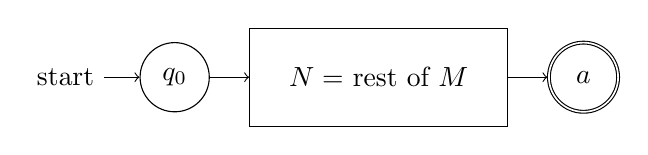
\begin{tikzpicture}[node distance=2cm]
    \node[state, initial](q0) {$q_0$};
    \node[draw, rectangle, inner sep=0.5cm](m) [right=0.5cm of q0] {$N = $ rest of $M$};
    \node[state, accepting](a) [right=0.5cm of m]{$a$};
    \path[->]
    (q0) edge (m)
    (m) edge (a);
  \end{tikzpicture}
\end{center}
Draw diagrams to show how to convert the regular expression you found in the previous problem to a DFA or NFA that recognises \(L'\).
Justify your answer fully, showing your steps.
Again, your answer is allowed to contain the schematic shown above.
\end{enumerate}
\begin{solution}
\begin{center}
\includegraphics[width=.9\linewidth]{assets/final-composite-machine.png}
\end{center}
\end{solution}
\item Question (10 points total)
\label{sec:org545bfac}
Let \(\Sigma = \{0,1\}\). Let \(L\) be the language consisting of all strings that have length at least two, and a \(1\) in the second spot from the right hand end.
That is,
\[L = \{w \mid w = a1b \text{ for some }a \in \Sigma^*\text{ and }b \in \Sigma\}.\]
\begin{enumerate}
\item (3 points) Draw a DFA or an NFA that recognises \(L\). No justification is required.
\begin{solution}
Here is an NFA.
\begin{center}
  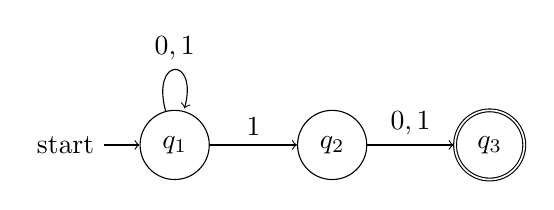
\begin{tikzpicture}[node distance=2cm]
    \node[state, initial] (q1) {$q_1$};
    \node[state] (q2) [right of=q1] {$q_2$};
    \node[state, accepting] (q3) [right of=q2] {$q_3$};
    \path[->]
    (q1) edge[loop above] node {$0,1$} ()
    (q1) edge node[above]{$1$} (q2)
    (q2) edge node[above]{$0,1$} (q3)
    ;
  \end{tikzpicture}
\end{center}
\end{solution}

\item (7 points) Convert your DFA or NFA into a regular expression. Show your work in every step.
\begin{solution}
First let us add a dummy start state \(s\) and a dummy accept state \(a\) as usual.
Then we remove each state in order.
\begin{enumerate}
\item Let's first remove \(q_1\). In this case, the label on \(s \to q_2\) gets updated to become \((0|1)^*1\)
\item Next let us remove \(q_2\). In this case, the label on \(s \to q_3\) gets updated to become \((0|1)^*1(0|1)\).
\item Finally let us remove \(q_3\). In this case, the label on \(s \to a\) gets updated to become \((0|1)^*1(0|1)\).
\end{enumerate}
The final answer is \((0|1)^*1(0|1)\).
\end{solution}
\end{enumerate}
\item Question (15 points total)
\label{sec:org7cd6644}
Consider the game of kayles, which is played as follows. There is a row of bowling pins, such as the following.
\[(\bullet \quad \bullet \quad \bullet \quad \bullet \quad \bullet)\]
A move consists of knocking out either a single pin, or two consecutive pins (without any gaps in between). For example, from the configuration above, the following are two of the possible valid moves.
\[(\bullet \quad \circ \quad \bullet \quad \bullet \quad \bullet)\quad \text{or}\quad (\bullet \quad \circ \quad \circ \quad \bullet \quad \bullet)\]
After the first move shown above, the first pin is not considered adjacent to the third pin. Similarly, after the second move shown above, the first pin is not considered adjacent to the fourth pin.
The player to knock out the last pin wins.

In the following problems, for convenience, you can write the original position as \((5)\), and the two new positions shown as \((1,3)\) and \((1,2)\), etc. Positions written this way can be considered to be the same up to reordering.

\begin{enumerate}
\item (3 points) Find a simple winning strategy for the game of kayles that has \(2022\) bowling pins in a single row. Explain briefly in words.

\item (7 points) Let \(G\) be the game of kayles with \(4\) pins in a row. Draw the game graph, and clearly label the Grundy value for each state in the game graph. No other justification is needed.
\begin{solution}
Here is the solution. A game position \(abc\) denotes a block of \(a\) pins followed by a block of \(b\) pins followed by a block of \(c\) pins, for example.

\begin{center}
\includegraphics[width=0.6\textwidth]{fe-kayles.png}
\end{center}
\end{solution}
\item (5 points) Consider the game \(G + H\), where \(G\) is the game state from the previous problem, and \(H\) is a game of nim with starting position \(7, 9, 12, 16\). Either find (with justification) at least one winning move for \(G + H\), or justify why it is a \(P\) position. Show your work.
\begin{solution}
The game \(H\) has Grundy value as follows.
We have \(7 = 111_2\), \(9 = 1001_2\), \(12 = 1100_2\) and \(16 = 10000_2\).
So the nim sum \(10010_2 = 18\).

The game \(G + H\) has Grundy value \(1_2 \oplus 10010_2 = 10011_2 = 19\).

A winning move is one where the Grundy sum becomes zero. For example one in \(H\) so that the new nim sum becomes \(1_2\).
In this case, we can achieve that if we change the pile of size \(16\) to a pile of size \(3\).
\end{solution}
\end{enumerate}
\end{enumerate}
\subsection{Another old final examination}
\label{sec:org904953a}
\toggletrue{solutions}
\subsubsection{Questions}
\label{sec:org64e6f79}
\begin{enumerate}
\item (20) True or False
\label{sec:org3c2c52a}
\begin{enumerate}
\item There is an integer \(a\) such that \(a^2 \equiv 2\) modulo \(10\).
\begin{solution}
False.  The squares modulo 10 are \(1, 4, 9, 6, 5\)
\end{solution}
\item The empty set has exactly one subset.
\begin{solution}
True
\end{solution}
\item Consider a directed graph with \(14\) vertices. If \(a\) and \(b\) are vertices in the graph, it is possible for there to be a path from \(a\) to \(b\) of length \(17\).
\begin{solution}
True
\end{solution}
\item Let \(P\) be a poset and \([x,y]\) an interval in the poset. If \(a, b \in [x,y]\) then \(a\) and \(b\) must be related under the poset relation.
\begin{solution}
False (but we have not talked about intervals, so you may ignore this).
\end{solution}
\item If the union of two languages is regular, then both of the languages have to be regular.
\begin{solution}
False.
\end{solution}
\item Any NFA must have at least one accept state.
\begin{solution}
False.
\end{solution}
\item There exists a regular expression \(r\) on \(\Sigma = \{a,b,c\}\) such that \(L(r)\) has exactly \(4\) elements.
\begin{solution}
True.
\end{solution}
\item The nim games \(G_1 = (1,2)\) and \(G_2 = (3)\) are equivalent.
\begin{solution}
True.
\end{solution}
\item The \(15 \times 15\) game of chomp is an \(N\) position.
\begin{solution}
True.
\end{solution}
\end{enumerate}
\item (15 or more) Short answers
\label{sec:orge857711}
\begin{enumerate}
\item (3 points) Write an example of a relation on \(\{1,2,3\}\) that is reflexive and symmetric, but not transitive. Justification is not required.
\begin{solution}
\(\{(1,1), (2,2), (3,3), (1,2), (2,3), (2,1), (3,2)\}\)
\end{solution}
\item (3 points) Consider the relation
\[\{(x,y) \in \mathbb{Z} \times \mathbb{Z} \mid (x-y)\text{ is a multiple of 7}\}.\]
List all equivalence classes \([x]\) such that
\[[x^2] = [1].\]
Justification is not required.
\begin{solution}
\([1]\) and \([-1]\).
\end{solution}
\item (3 points) Draw any directed graph with exactly \(4\) vertices and at least 4 edges, whose adjacency matrix squares to zero. Justification is not required.
\begin{solution}
Just make sure that you do not have paths of length 2.
\end{solution}
\item (3 points) Let \(\Sigma = \{0,1\}\). Let \(r = 0(11|0)^{\ast}(00|1)^{\ast}\).
Among the following strings, which ones (if any) are accepted by \(r\)? List just the ones that are accepted; justification is not required.
\[\epsilon, \quad 0111,\quad 011110011, \quad 0010,\quad 1100,\quad 110111.\]
\begin{solution}
Left to you.
\end{solution}
\item (3 points) Draw any NFA or DFA whose language is non-empty but finite. Justification is not required.
\begin{solution}
NFA that only accepts \(0\): two states \(A\) (start state) and \(B\) (accept state) with only one arrow \(A \to B\) labelled \(0\).
\end{solution}
\end{enumerate}
\item (10) Relations etc
\label{sec:org6f750c8}
\begin{enumerate}
\item (4 points) Consider the equivalence relation
\[\{((a,b),(c,d)) \in \mathbb{R}^2 \times \mathbb{R}^2 \mid \min\{a,b\} = \min\{c,d\}\}.\]
Choose any \emph{specific} point \((a,b)\), and sketch its equivalence class.
Show your work.
\begin{solution}
The equivalence classes are ``L''-shapes centred at points of the form \((x,x)\).
\end{solution}
\item (3 points) Consider a binary operation on the set of equivalence classes of the previous relation, defined as \[[(a,b)] \star [(c,d)] = [(a,c)].\]
Explain with a counterexample why this operation is not well-defined.
\begin{solution}
The result \([(a,c)]\) changes if we change the representatives \((a,b)\) and \((c,d)\).
For example, take \((a,b) = (2,1)\) and \((c,d) = (2,3)\), then \((a,c) = (2,3)\).
But if we change \((a,b)\) to \((1,2)\), which is equivalent to \((1,2)\), then we get \((a,c) = (1,3)\), which is not equivalent to \((2,3)\).   
\end{solution}
\item (3 points) Consider the relation \(\{(a,b) \in \mathbb{Z} \times \mathbb{Z} \mid a + b \neq 1\}\).
Is this an equivalence relation? Why or why not? Explain your answer.
\begin{solution}
This relation is not transitive: \((0,2)\) and \((2,1)\) are in the relation but \((0,1)\) is not.
\end{solution}
\end{enumerate}
\item (10) Graphs
\label{sec:org3283501}
Consider the graph shown below.
\begin{center}
\includegraphics[width=0.6\textwidth]{final-12.png}
\label{orga03d77f}
\end{center}
\begin{enumerate}
\item (3 points) Draw the transitive closure of this graph, ignoring the weights. Justification not required.
\begin{solution}
\begin{center}
\includegraphics[width=.4\textwidth]{final-transitive.png}
\label{org63cff44}
\end{center}
\end{solution}

\item (7 points) Write down the weighted adjacency matrix using the weights shown in the diagram. Paths of length zero are considered to have weight zero. Calculate the matrix that shows the minimum weight paths between any pair of vertices. Show your work.
\begin{solution}
The weighted adjacency matrix is
\[ W = \begin{pmatrix}
   0&1&1&\infty\\
   \infty&0&3&\infty\\
   \infty&\infty&0&2\\
   1&5&\infty&0
   \end{pmatrix}. \]
The minimum-weight path can be computed by the min-plus cube of this matrix.
We have
\[W^{\odot 2} = 
   \begin{pmatrix}
   0&1&1&3\\
   \infty&0&3&5\\
   3&7&0&2\\
   1&2&2&0
   \end{pmatrix},
   \]

and
\[W^{\odot 3}
   \begin{pmatrix}
   0&1&1&3\\
   6&0&3&5\\
   3&4&0&2\\
   1&2&2&0        
   \end{pmatrix}.\]
\end{solution}
\end{enumerate}
\item (8) Posets
\label{sec:org48012cc}
Consider the poset whose Hasse diagram is shown below.
Answer the following questions about this poset.
\begin{center}
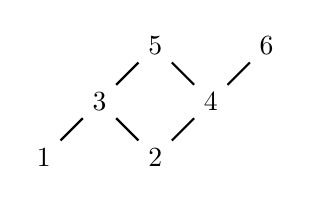
\begin{tikzpicture}
\node (A) at (0,0) {5};
\node[below left of=A] (C) {3};
\node[below right of=A] (D) {4};
\node[above right of=D] (B) {6};
\node[below left of=C](E) {1};
\node[below right of=C](F) {2};
\draw[thick] (A) --  (C) -- (E);
\draw[thick]  (C) -- (F) -- (D);
\draw[thick] (A) -- (D) -- (B);            
\end{tikzpicture}
\end{center}
\begin{enumerate}
\item Write all the maximal elements.
\item Write all the minimal elements.
\item Does the poset have a rank function? If yes, write one.  If not, why not?

\begin{solution}
\begin{enumerate}
\item Maximal elements: 5, 6
\item Minimal elements: 1, 2
\item There is a rank function: set \(f(1) = f(2) = 0\); \(f(3) = f(4) = 1\); \(f(5) = f(6) = 3\).
\end{enumerate}
\end{solution}
\end{enumerate}
\item (15) Languages
\label{sec:org3316828}
Let \(L\) be the language on \(\Sigma = \{0,1\}\) defined as follows:
\[L = \{\text{words, including the empty word, that alternate \(0\)s and \(1\)s}\}.\]
\begin{enumerate}
\item (4 points) Draw either a DFA or an NFA that recognises exactly the language \(L\). No justification required, but all labelling must be clear.
\item (9 points) Convert the machine that you drew in the previous part into an equivalent regex via the state-deletion method discussed in class. Draw and clearly label each step, but no other justification is required.
\item (2 points) Let \(L'\) be the language
\[L' = \{\text{words, including the string \(1\), that begin and end with \(1\)}\}.\]
Write down a regex whose language is \(L \cap L'\). Justification not required; just write down your answer.
\end{enumerate}
\begin{solution}
\begin{enumerate}
\item Here is an NFA.
\begin{center}
\includegraphics[width=.3\textwidth]{assets/Another_old_final_examination/2025-11-04_14-56-18_screenshot.png}
\end{center}
\item We have to first sanitise the NFA and then apply the state-deletion method.
\begin{center}
\includegraphics[width=.6\textwidth]{assets/Another_old_final_examination/2025-11-04_15-04-13_screenshot.png}
\end{center}

So the regex is  \(\epsilon | 0(10)^{*}(\epsilon | 1) | 1(01)^{*}(\epsilon | 1)\)

\item The intersection is words that begin with \(1\), alternate, and then end with \(1\).
This is \(1(01)^{*}\).
\end{enumerate}
\end{solution}
\item (15) Games
\label{sec:org1e5a29b}
The \emph{divisors game} is played as follows. The starting state is the set \(D_n\) of all divisors of some fixed positive integer \(n\), not including \(n\) itself.
   For example, the starting state for \(n = 12\) is the set \(D_{12} = \{1,2,3,4,6\}\).

A move consists of deleting one of the elements of the set along with all of its divisors, to give another finite (possibly empty) set of positive integers.
Here are some examples of valid moves:
\begin{align*}
  \{1,2,3,4,6\} &\xrightarrow{\text{remove }1} \{2,3,4,6\},\\
  \{1,2,3,4,6\} &\xrightarrow{\text{remove }3} \{2,4,6\},\\
  \{1,2,3,4,6\} &\xrightarrow{\text{remove }6} \{4\}.
\end{align*}
The person who cannot make a move loses.

\begin{enumerate}
\item (7 points) Consider the divisors game starting at \(D_n\) for \(n = 12\). That is, your starting state is \(\{1,2,3,4,6\}\).
Draw the game graph starting from this state, and label each state clearly with its Grundy value. No justification required but the labels must be clear.

\emph{(Hint: To help you check your work, the Grundy value of the state \(\{3,4,6\}\) is \(3\).)}

\item (4 points) Let \(G\) be the divisors game starting at \(D_6 = \{3,4,6\}\).
Recall that the Grundy value of \(G\) is \(3\).
Let \(H\) be the nim game starting at the state \((2,3,4)\).

Is \(G + H\) an \(N\) position or a \(P\) position?
If you think that \(G + H\) is a \(P\) position, explain why.
If you think that \(G + H\) is an \(N\) position, write down (with a brief explanation) an optimal move that the first player should make in the game \(G + H\).

\item (2 points) Draw the Hasse diagram of the set \(D_{16} = \{1,2,4,8\}\) with the divisibility relation. No justification required.

\item (2 points) Find the Grundy label of the start state for \(n = 2^{2023}\). That is, the starting state for the game would be \(D_n = \{1, 2, 2^2, \ldots, 2^{2022}\}\). No justification required; just write down your answer.

\emph{(Hint: what does the game graph for the starting state \(D_{16}\) look like? Try to extrapolate from this.)}

\begin{solution}
\begin{enumerate}
\item The Grundy values are in red.  I have abbreviated the states by dropping commas and braces.
\begin{center}
\includegraphics[width=.5\textwidth]{assets/Another_old_final_examination/2025-11-04_15-10-57_screenshot.png}
\end{center}
\item \(\operatorname{Nim}(2,3,4)\) has Grundy value \(2 \oplus 3 \oplus 4 = 10 \oplus 11 \oplus 100 = 101 = 5\).
Then \(G + H\) has Grundy value \(3 \oplus 5 = 11 \oplus 101 = 110 = 6\), which is non-zero.
So \(G+H\) is an \(N\)-game.

There are two kinds of optimal moves: move \(G\) to a state with Grundy value \(11 \oplus 110 = 101\) (not possible as seen from the graph above), or \(H\) to a state with Grundy value \(101 \oplus 110 = 11\), which must be possible.
To figure out how to achieve this, we xor 110 with the Grundy values of each nim-stack, and see which ones lead to a smaller stack.  The only stack in which this happens is the third one: \(110 \oplus 100 = 10\); so we have to move the 4-pile to a 2-pile.

\item This is just a vertical line.

\item \(D_n\) is just a single pile nim of size \(2023\).
So the Grundy label is \(2023\).
\end{enumerate}
\end{solution}
\end{enumerate}
\end{enumerate}
\end{document}
